%%%% Various options for document class.
%%\documentclass[usenatbib, a4paper, 11pt]{aastex}
%%\documentclass[preprint, 11pt, a4paper]{aastex}
%%\documentclass[twocolum]{revtex4}
%%\documentclass{report}
%\documentclass[useAMS,usenatbib]{mn2e_x}
\documentclass[preprint, a4paper, 11pt]{aastex}
%\usepackage{psfig,morefloats,url}
%use preprint2 for 2 columns paper.

%% declare any packages used
\usepackage{graphicx}
\usepackage{natbib}
\usepackage{graphicx}
\usepackage{color}
\usepackage{pdfpages}
\usepackage{appendix}
\usepackage{subfigure}
\usepackage{url}
%\usepackage{pngfig}
%\usepackage[dvips]{color}
%\usepackage{aabib}


%\marginparwidth = 25pt
\citestyle{aa}
\addtolength{\topmargin}{-.5in}
%\addtolength{\bottommargin}{-1in}
%% This command added as margins are wrong in mn2e, it appears. 
%% Not needed for other classes
\usepackage{float}



%%%%%%%%%%%%%%%%%%%%%%%%%%%%%%%%%%%%%%

\begin{document}
%% define bibstyle and other definitions
\bibliographystyle{aabib}
%% renew commands
%%\renewcommand{\labelitemi}{$.$}

%% Codes
\def\py{\textsc{Python}}
\def\tar{\textsc{Tardis}}
\def\cld{\textsc{Cloudy}}
\def\agn{\textsc{Agnspec}}


%% Lines and ions
\def\civ{C~\textsc{iv}}
\def\nv{N~\textsc{v}}
\def\hei{He~\textsc{i}}
\def\heii{He~\textsc{ii}}
\def\mg{Mg~\textsc{ii}}
\def\al{Al~\textsc{iii}}
\def\heii{He~\textsc{ii}}
\def\ovi{O~\textsc{vi}}
\def\la{Ly~$\alpha$}
\def\ha{H~$\alpha$}
\def\hb{H~$\beta$}



%% Journal definitions
\def\araa{ARAA}
\def\nat{Nature}
\def\apjl{ApJ Letters}
\def\aapr{AAPR}
\def\ssr{SSR}
\def\apj{ApJ}
\def\apjs{ApJs}
\def\pasp{PASP}
\def\aap{A\&A}
\def\mnras{MNRAS}
\def\aj{AJ}
\def\rmxaa{RMXAA}
\def\aaps{A\&As}

%%%%%%%%%%%%%%%%%%%%%%%%%%%%%%%%%%%%%%
%
%          TITLE AND AUTHORS
%
%%%%%%%%%%%%%%%%%%%%%%%%%%%%%%%%%%%%%%%

\title
{
% Modelling quasar outflows:
% clumpy winds and broad emission lines
Unifying quasars with clumpy wind models
}


% [Matthews, J.]
% \author[Matthews, J.]{James Matthews \\
% {\sl  Supervisor: Prof. Christian Knigge} \\
% {\sl School of Physics \& Astronomy, University of Southampton,
%   Southampton, SO17 1BJ, UK}}

%\author[Matthews et al.]
\author{
\parbox[t]{\textwidth}{
J.~H.~Matthews$^1$\thanks{jm8g08@soton.ac.uk}, C.~Knigge$^1$,
N.~Higginbottom$^1$, K.~S.~Long$^2$, S.~A.~Sim$^3$ and S.~W.~Mangham$^1$
}
\medskip  
\\$^1$School of Physics and Astronomy, University of Southampton, Highfield, Southampton, SO17 1BJ, United Kingdom
\\$^2$Space Telescope Science Institute, 3700 San Martin Drive, Baltimore, MD, 21218
\\$^3$School of Mathematics and Physics, Queens University Belfast, University Road, Belfast, BT7 1NN, Northern Ireland, UK
}

\date{\today}
%\\
%Supervisor: Prof. Christian Knigge\\
%{\sl School of Physics \& Astronomy, University of Southampton,
%  Southampton, SO17 1BJ, UK}}


%%%%%%%%%%%%%%%%%%%%%%%%%%%%%%%%%%%%%%
%
%          ABSTRACT
%
%%%%%%%%%%%%%%%%%%%%%%%%%%%%%%%%%%%%%%%




\begin{abstract} 
% Broad absorption lines (BALs) in the ultraviolet 
% are seen in $\sim20\%$ of quasi-stellar objects (QSOs). 
% Blue-shifted broad absorption lines (BALs) are the most direct evidence of 
% accretion disc `winds' in such systems; mass loaded outflows
% emanating from the disc that may be driven by line forces or
% magnetic processes. 
Various unification schemes for
quasars and luminous active galactic nuclei (AGN) have proposed
that the broad emission line region is roughly cospatial
with broad absorption line (BAL) gas and much of the phenomenology of luminous AGN
can be explained by a simple geometrical picture involving an accretion
disc and associated outflow. Here, we test this paradigm by 
utilising our state-of-the-art radiative transfer code to produce synthetic spectra
from simple biconical disc wind models. In particular, we expand on our previous 
work in which a benchmark model for BAL quasars was produced. 
We have conducted a limited parameter search with the aim of unifying quasar phenomenology,
and arrive at an improved model. The grid is now publicly available.
We find that a simple treatment of clumping (`microclumping') 
allows for a more realistic X-ray luminosity in the model by lowering the 
ionization parameter. We examine the X-ray properties of this new model
and find good agreement with existing X-ray samples of AGN and QSOs.
We find that the dense, X-ray heated wind 
produces strong H recombination and collisionally excited resonance 
line emission to emerge at the low inclination angles, 
which represent quasars within this unification scenario.
% We also treat Hydrogen using a `macro-atom' approach in order to 
% examine the effect of recombination on Hydrogen emission lines, and
% this results in significant line emission in Lyman~$\alpha$ and the Balmer series.
However, we are unable to reproduce the remarkably similar of line-to-continuum
ratios between BAL and non-BAL quasar composites.
This is due to a fundamental constraint arising
from the anisotropy of emission from a classical thin disc. 
We briefly explore the effect of relativistic beaming, gravitational redshift and 
light bending on the angular distribution of disc continuum emission. 
We find that these general relativistic effects do cause the disc to
emit slightly more isotropically, but this is not yet sufficient to produce a
self-consistent model. We discuss wind reprocessing as a potential solution.
Overall, our work suggests that geometric unification
involving an accretion disc wind is a promising scenario, but our results 
pose a number of difficult challenges to such a model.
% Determining the true geometry of ADWs and uncovering the true disc spectral 
% (and angular) energy distribution are key next stpng if we are to build up a 
% holistic picture of the quasar population.
\end{abstract}

\maketitle
%\begin{keywords}
%AGN: outflows
%\end{keywords}



%%%%%%%%%%%%%%%%%%%%%%%%%%%%%%%%%%%%%%
%
%          INTRODUCTION
%
%%%%%%%%%%%%%%%%%%%%%%%%%%%%%%%%%%%%%%%

\section{Introduction}

% Introduction focussing on key points
% \begin{itemize}
% \item standard wind + BALQSO introduction
% \item focus on unification and that we are testing it
% \item some discussion of scales, referencing e.g. reverb maps, variability, microlensing, Arav 
% \item clumping background: stellar winds, clumping in AGN winds, variability
% \end{itemize}

The spectra of 
quasars and luminous active galactic nuclei (AGN) 
typically exhibit a series of strong emission lines
with an underlying blue continuum - the so-called {\sl `big blue bump'} (BBB). 
The BBB is normally attributed to emission from a geometrically thin, 
optically thick accretion disc surrounding the central black hole (REF), similar
to that described by \cite{shakurasunyaev1973}.
In addition to the inflowing accreting material, 
outflows are ubiquitous in AGN
and quasars \citep{kellerman1989,ganguly2008}. These outflows can take the form of 
highly collimated radio jets \citep[e.g.][]{hazard1963,potash1980,perley1984,marscher2006}, 
or mass-loaded `winds' emanating from the accretion disc 
\citep{weymann1991,turnermiller2009}. 
Outflows in AGN offer a 
potential feedback mechanism through which the central source can 
affect its environment \citep{king2003,king2005,fabian2012}
-- feedback that is required in models of galaxy evolution (REFs) 
and may explain the `$M-\sigma$' relation \citep{silkrees1998,haring2004}.

Approximately $20\%$ of quasars exhibit blueshifted ($\sim 0.1c$)
broad absorption lines (BALs) in the ultraviolet,
providing clear evidence for outflowing absorbing material
\citep{weymann1991, reichard2003, knigge2008, turnermiller2009, allen2011}.
The simplest explanation for the incidence of 
BAL quasars (BALQSOs) is in terms of an accretion disc wind (ADW). 
Within this paradigm, the BALQSO fraction is associated with
the covering factor of the outflow.
In addition, ADWs may offer a natural explanation for the
diverse phenemonology of luminous AGN and QSOs \citep[e.g.][]{MCGV95, elvis2000}. 
In such a model, a biconical wind rises from 
the accretion disc, and the class of object is explained by the material
intercepting the line of sight. Depending on viewing angle, an observer 
may then see a BALQSO or normal `Type 1' quasar.
Within this framework, the broad-line region (BLR) is normally
assumed to correspond to the dense wind base.
There are various spectroscopic sub-classifications of BALQSOs: 
HiBALQSOs, which only exhibit higher
ionization line absorption; LoBALQSOs which also show
absorption in lower ionization state species such as \mg\ and \al; and
FeLoBALQSOs which show further absorption in Fe~\textsc{ii} and \textsc{iii}.
In unified models, this is generally attributed to ionization stratification
of the outflow \citep[e.g.][]{elvis2000}.

% As well as acting as a source of photoionized plasma, a 
As well as imprinting clear line absorption features,
disc winds may also have a profound effect on the structure and 
emergent {\em continuum} of the accretion disc itself.
Mass-loss will alter the accretion rate and resultant 
temperature of the accretion disc, possibly explaining some 
of the features we typically see in luminous AGN \citep{laordavis2014}.
Recent results from \cite{capellupo2015} find 
that if one includes a combination of mass-loss, general relativity (GR) and Comptonisation
then AGN spectral energy distributions (SEDs) can, in general, be fitted well with accretion disc models.
Mass-loss therefore appears to be critical if an $\alpha$-disc
model is to successfully fit AGN SEDs, particular in the UV region of the spectrum.

Despite the clear importance of ADWs in understanding AGN SEDs and accretion physics, 
much of the underlying outflow physics remains highly uncertain. 
Several possible driving mechanisms for ADWs have been proposed, including
thermal pressure \citep{weymann1982, begelman1991}, magnetocentrifugal forces 
\citep{blandfordpayne,pelletier_pudritz} and 
radiation pressure on spectral lines \citep[`line-driving';][]{lucysolomon1970,shlosman1985,MCGV95}.
Of these, line-driving is possibly the most attractive, as
strong absorption lines are already seen in BALQSOs and the X-ray spectra of AGN 
\citep{reeves2003,poundsreeves2009,tombesi2010a}.
The presence of line-locked features \citep{bowler2014} 
and the `ghost of \la' (Arav et al. 1996; Arav 1996; North 2006; but see 
also Cottis et al. 2010) \nocite{arav1995, arav1996, north2006,cottis2010}
in the spectra of some BALQSOs also gives clearer evidence that line-driving is
at least partially contributing to the acceleration of the wind.

The efficiency of line-driving is crucially dependent on the ionization state 
of the outflowing plasma, meaning that it is difficult to prevent 
the wind becoming over-ionized and `failing' in the presence of strong X-rays. 
\cite{MCGV95} proposed a potential solution: 
a region of `hitchhiking gas' that could shield the wind from the central X-ray source. 
Hydrodynamic simulations of line-driven disc winds also found a shielding region
was required to maintain the correct ionization state \citep{PSK2000,PK04}. 
However, \cite{H14} showed that including multiple scattering means the ionizing radiation 
field could still reach the previously shielded regions in those particular models.
An alternative solution is that the wind is clumped \citep[e.g.][]{hamann2013}
possibly on multiple scale lengths. Local density enhancements could lower the 
ionization parameter of the plasma while still maintaining the same mass-loss 
rate and column density. 


Evidence for dense substructures in AGN winds is widespread.
BALQSOs show complex absorption line profiles \citep{ganguly2006, simonhamann2010}
and exhibit variability in these profile shapes \citep{capellupo2011,capellupo2012,capellupo2014}.
AGN generally show variability in X-ray absorption components \citep[e.g.][]{risaliti2002}
and many models for the BLR consist of clumps embedded in an outflow 
\citep{krolik1981, emmering1992, dekool1995, cassidyraine1996}.
Clumping can be caused by magnetic confinement \cite{dekool1995},
or the instabilities inherent to line-driven winds 
\citep{lucysolomon1970,macgregor1979,carlberg1980,owockirybicki1984,owockirybicki1985}.
Additionally, clumping is required in line-driven hot star winds 
in order to explain observations \citep{hillier1991eswingsmodel}. Complex substructures 
on a variety of scales are also produced in simulations of line-driven 
outflows in AGN \citep{PSK2000,PK04,progakurosawa2010,proga2014}.
Clumpy winds therefore offer an observationally motivated and theoretically 
predicted way to lower the ionization state of a plasma, possibly in tandem
with a shielding scenario. 




% An inhomogenous outflow has been proposed as a model for the BLR (REFs)
% Clumping is expected in outflows and BLRs.


% The UV spectrum of {\em non-BAL} QSOs is typified by a series
% of strong emission lines (e.g. \la, \civ, \nv) with an underlying blue continuum
% - the so-called {\sl `big blue bump'} (BBB). The BBB is normally attributed to blackbody-like
% emission from an accretion disc surrounding the central black hole (REF), similar
% to that described by \cite{shakurasunyaev1973}. However,
% a number of issues have arisen relating to this model. First, 
% AGN/QSO spectra exhibit a `break' in the spectrum at around $1000$~\AA 
% which scales only weakly with black hole mass. This potentially 
% suggests a problem with a thin disc model (e.g. Antonucci). 
% However, it is possible that this is the result of incorrect intergalactic medium
% (IGM) corrections (REF) or corresponds to the temperature 
% at which a line-driven wind carries mass away from the system (laor davis).
% Second, results from microlensing (REFs) imply that the disc emission 
% region is $\sim4$ times larger than one might expect from a Shakura-Sunyaev
% model. Inhomogenous discs have been proposed as an alternative (REFs).
% These observations appear to pose problems for the thin disc model of luminous,
% sub-Eddington AGN. However, recent results from \cite{capellupo2015} find 
% that if one includes a combination of mass-loss, general relativity (GR) and Comptonisation
% then AGN SEDs can, in general, be fitted well with accretion disc models.
% Uncovering the intrinsic disc SED and understanding the effect of the outflow on the accretion 
% mechanism is clearly crucial if we are to properly understand the physical nature
% of AGN.

% The geometry and size of the BLR is also a matter of contention. 
% The main constraints on the emission region size come from microlensing (REFs)
% and reverberation mapping (REFs). While these observations have mostly been
% carried out for Seyfert galaxies, there are also a few instances of these methods
% being applied to quasars (REFs). A number of different proposals have been made 
% for the origin of the BLR. Early AGN unification scenarios posited that the broad emission lines
% where produced by clouds of plasma orbiting fairly close to the BH (refs).
% Since then, multiple interpretations of a disc wind model have been proposed,
% with varying radii and geometries (refs). 

There has been some success using simple
kinematic prescriptions for biconical disc winds to model 
AGN and quasar outflows \citep[][hereafter H13]{simlong2008,sim2010,higginbottom2013}. 
H13 successfully produced a benchmark model for BALQSOs. However, the model
had two key drawbacks. Firstly, an unrealistically low X-ray luminosity
was required in order to prevent over-ionization of the outflow.
Secondly, the model failed to produce the strong emission lines 
required at low inclinations in a unified model.
In this paper, we attempt to address these issues, and test the disc wind 
unification model using Monte Carlo radiative transfer (MCRT) and photoionization 
calculations. The paper is organised as follows.
In section 2, we describe some of the important photoionization 
and MCRT aspects of the code. In section 3, we outline the model, including 
a description of our clumping implementation. In section 4, we present the results 
from a clumped model. In section 5 we discuss our results, 
focussing particular on the anisotropy of 
disc emission and GR effects, and finally, in section 6, we summarise our findings.



%  a simple model in which
% quasars are unified by BH mass, Eddington ratio and viewing angle can successfully
% reproduce UV, optical and X-ray properties of {\em both} 
% BALQSO's and normal emission line quasars. 

% Geometrical unification pictures have suggested that 
% the BAL fraction can be interpreted as the covering factor
% of an accretion disc wind (refs), and some also propose
% that this disc wind may also be the source of the broad emission
% lines (BELs) seen in QSOs (refs). 
% Alternatively, there are a number of evolutionary models in which
% QSOs spend approximately $20\%$ of their lifetime as BALQSOs in which the outflow
% has a high covering factor (refs). 
% It is also possible that BALQSOs lie in a distinct region
% in terms of Eddington ratio (refs), but this is somewhat refuted 
% by observations (refs). % to e.g. Allen and Eigenvector I papers Ledd of BALQSOs
% Orientation, evolution, black hole mass and eddington ratio 
% may all have an effect on the BAL fraction (refs),  % to e.g. Allen
% and the importance of each must be understood to build up coherent picture.


% The driving mechanism for accretion disc winds is uncertain. The winds responsible 
% for BALs must at least have some line-driven component,
% as very strong resonance lines exert a strong line force on the 
% gas (refs). Line-driven winds are notoriously unstable 
% \citep{lucysolomon1970,macgregor1979,owockirybicki1984,owockirybicki1985}.
% meaning that one may expect an unstable and inhomogenous 
% velocity and density structure (refs). Magnetically driven
% winds may also produce clumpy winds or `clouds' of material which
% are magnetically confined (refs here to Shlosman, Begelman and the like).
% Describe mechanism.

% Evidence for an inhomogenous density structure in an accretion disc wind 
% and/or the broad emission line region comes from multiple sources. 
% Microlensing observations of absorption troughs suggest that different lines of sight 
% exhibit varying velocity components (refs), and BALQSO troughs 
% are known to exhibit variability (refs).

% trend of L_X with radio jets and Sy 1s
% trend of BALs with radio loudness
% see MCGV95






%%%%%%%%%%%%%%%%%%%%%%%%%%%%%%%%%%%%%%%%%%%%%%%%%

% MCRT

%%%%%%%%%%%%%%%%%%%%%%%%%%%%%%%%%%%%%%%%%%%%%%%%%

\section{Ionization and Radiative Transfer}

We use the MCRT code \py\ to carry out our radiative transfer and photoionization
calculations in non-local thermodynamic equilibrium (non-LTE). 
The has been used to model accreting white dwarfs 
(Long \& Knigge 2002, hereafter LK02; Noebauer et al. 2010; 
Matthews et al. 2015, hereafter M15), young-stellar objects \citep{simmacro2005}
and quasars (H13). \nocite{noebauer, M15, LK02}
These studies contain extensive detail on the code, 
so we only briefly describe the key elements of the global 
ionization calculation and other important aspects.

\subsection{Line transfer}

To treat line transfer, we adopt the same hybrid scheme 
described by M15, 
in which the energy flows
through the system are described in terms of indivisible
energy quanta of radiant or kinetic energy 
(`$r-$packets' and `$k-$packets' respectively; see also section 2.3).
These energy packets interact with either two-level `simple ions'
or full `macro-atoms'. The macro-atom implementation 
is described in full by \cite{lucy2002, lucy2003}.
Our scheme allows one to treat non-LTE line transfer in radiative equilibrium
without approximation for elements which are identified as 
full macro-atoms, while maintaining the fast `two-level' 
treatment of resonance lines when elements are identified 
as simple-ions (see M15). In this study,
only H \& He are treated as macro-atoms, because 
we expect recombination to be important
in determining their level populations and resultant line emission.

\subsection{Ionization Scheme}

Macro-atoms have their ion and level populations derived from
MC rate estimators as described by M15. Previously (LK02, H13, M15),
we adopted a modified Saha approach to calculate the ionization fractions
of simple-ions. We have now improved our code to explicitly solve the 
rate equations in between ions in non-LTE. 
Not only does this
dispense with a number of small assumptions made in the modified Saha approach, 
it is also more numerically stable, 
and in principle allows the direct addition of extra physical 
processes such as Auger ionization, which would have to be approximated 
if using the previous technique.

To avoid approximating the complex AGN SED as e.g. a dilute blackbody \citep[][M15]{ML93},
we model the SED in a cell using the technique described by H13. In this scheme,
the mean intensity in a series of bands is modeled as a normalised power law in 
frequency $\nu$
\begin{equation}
J_{\nu,j}=K_{pl}\nu^{\alpha_{pl}},
\end{equation}
for a band $j$, or an exponential 
\begin{equation}
J_{\nu,j}=K_{exp} e^{(-h\nu/k T_{exp})}.
\end{equation}
Here, $K_{exp}$, $K_{pl}$, $T_{exp}$ and $\alpha_{pl}$ are spectral fit parameters
deduced from the band-limited radiation field estimators.
The ionization rate out of ion $i$ can then be written as 
\begin{equation}
R_{i,i+1}(J)= 
\displaystyle{
n_i \left(C_{i} n_e + 
\sum_{band~j=0}^{n}~
{\int_{\nu_j}^{~\nu_j+1}{J_{\nu,j}\sigma_i(\nu)\nu^{-1}d\nu}}
\right),}
\end{equation}
where $\sigma_i$ is the photoionization cross-section and $C_{i}$
represents the collisional ionization coefficient.
The recombination rate {\em into} ion $i$ is simply given by 
\begin{equation}
R_{i+1,i}(T_e) = (\alpha^i_{RR} + \alpha^i_{DR} + \alpha^i_{CR}) n_{i+1} n_e
\end{equation}
Where each $\alpha^i$ here is the recombination rate coefficient into the ground state of ion $i$.
The subscripts denote radiative, dielectronic and 
collisional (three-body) recombination respectively.
We thus neglect recombination to and from excited states in the simple-ion calculation. 
For simple-ions, we use a dilute Boltzmann equation to calculate 
the population of level $k$ in ionic stage $j$,
\begin{equation}
\frac{n_{jk}}{n_j} = \frac{W g_k}{z_j(T_R)} \exp(-E_k/kT_R).
\end{equation}
Here $z_j$ is the partition function of ionic stage $j$,
$T_R$ is the effective radiation temperature,
$E_k$ is the energy difference between level $k$ and the ground state,
and $g_k$ is the statistical weight of level $k$. 

% We improve on this method by abandoning the modified Saha approach
% entirely, and instead computing the ionization state by 
% explicitly solving the rate equations in between ions in non-LTE. 
% Photoionization and recombination rates are calculated using MC estimators recorded
% during the photon propagation. Not only does this dispense with a number of
% small assumptions made in the modified Saha approach, it is also more numerically stable, 
% and in principle allows the direct addition of extra physical processes such as Auger ionization, which would have to be approximated if using the previous technique.
\subsection{Physical Processes}

We include all free-free, bound-free and bound-bound heating
and cooling processes in the model. For radiative transfer purposes
we treat electron scattering in the Thomson limit, 
but take full account of Compton heating and cooling when
calculating the thermal balance of the plasma (see H13).
Adiabatic cooling is included and represents the only
departure from strict radiative equilibrium, but is insignificant 
in most of the outflow.
% It is dealt with self consistently by the spontaneous destruction
% of $k$-packets with a probability

% \begin{equation}
% P_{\rm{adiabatic~destruction}} = \frac{C_{\rm{adiabatic}}}{C_{\rm{total}}},
% \end{equation}
% where $C_{\rm{adiabatic}}$ and ${C_{\rm{total}}}$ represent the 
% adiabatic and total cooling rates in the cell.


\subsection{Atomic Data}

We use the same atomic data as described by LK02 and since updated by H13 and M15, 
with the addition of direct ionization data from \cite{dere2007}. 
Photoionization cross-sections are from \textsc{Topbase} \citep{cunto1993} and  \cite{vfky}.
Dielectronic and radiative recombination rate coefficients are taken from 
the \textsc{Chianti} database version 7.0 \citep{dere1997,landi2012}.
We use ground state recombination rates from \cite{badnell2006} where available,
and otherwise default to calculating recombination rates from the Milne
relation. Free-free Gaunt factors are from \cite{sutherland1998}.


%%%%%%%%%%%%%%%%%%%%%%%%%%%%%%%%%%%%%%%%%%%%%%%%%

% MODEL DESCRIPTION

%%%%%%%%%%%%%%%%%%%%%%%%%%%%%%%%%%%%%%%%%%%%%%%%%


\section{A Clumpy Biconical Disk Wind Model for Quasars}

Our kinematic prescription for a biconical disc wind model
follows \cite{SV93}, and is described further by
LK02, H13 and M15. A schematic is shown in figure~\ref{fig:cartoon},
with key aspects marked. The general biconical
geometry is similar to that invoked by \cite{MCGV95} and 
\cite{elvis2000} in order to explain the phenomenonology
of quasars and BALQSOs.


\begin{figure} 
\centering
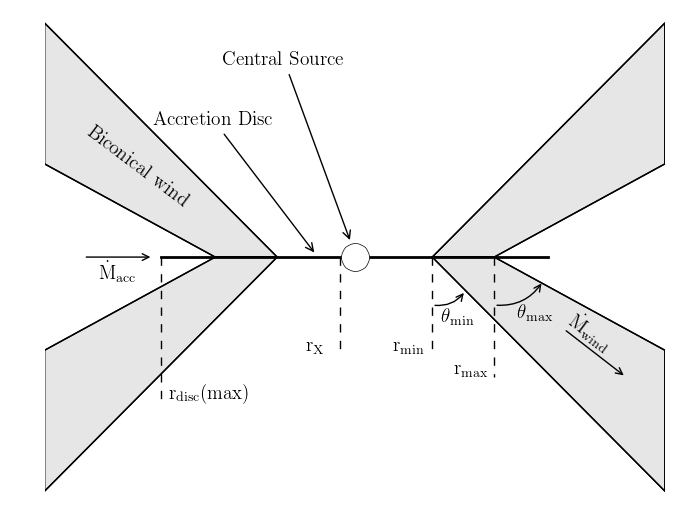
\includegraphics[width=0.45\textwidth]{figures/fig2_cartoon.png}
\caption
{
A cartoon showing the geometry and some key parameters of
our biconical wind model.
}
\label{fig:cartoon}
\end{figure} 



% \subsection{A Benchmark Model for BALQSOs}

% \cite{higginbottom2013} presented a benchmark model for
% (BAL)QSOs...introduce key parameters. 

\subsection{Photon Sources}

%Describe the photon sources in the model.

The accretion disc in our model is geometrically thin, but optically thick
and thus adopt a standard multi-temperature blackbody
using a \cite{shakurasunyaev1973} temperature profile. 

The emergent SED is thus determined by the specified accretion rate ($\dot{m}$)
and central BH mass ($M_{BH}$).
All photon sources in our model are assumed opaque, meaning
that photons which strike them are destroyed.
The inner radius of the disc extends to the innermost 
stable circular orbit (ISCO) of the BH. 
We assume a Schwarzchild BH with an ISCO at $6~R_G$.
The X-ray source in our model is treated as an isotropic sphere at the ISCO,
which emits r-packets according to a power law in flux with index $\alpha_X$ such that
\begin{equation}
F_X (\nu) = K \nu^{\alpha_X}.
\end{equation}
The normalisation, $K_X$ of this power law is such that it 
produces the specified 2-10~keV luminosity, $L_X$.
In addition to the disc and X-ray source, 
the wind is able to reprocess radiation. However, new 
photon packets are not produced in the wind (as in LK02). 
Instead, this reprocessing is dealt with by enforcing strict
radiative equilibrium ({\em modulo} adiabatic cooling)
via an indivisible energy packet
constraint (see Lucy 2002, M15; also section 2.3).
% \begin{equation}

% \end{equation}

% With a normalisation such that it produces the correct 2-10kev luminosity.

% Photons striking the 





% which successfully reproduced BAL features 
% in synthetic spectra using \py. However, the model
% had a few key drawbacks when considering its potential
% for unification. First, it failed to produce significant
% broad emission lines at non-BAL viewing angles; this is 
% a key requirement for a unified QSO model. Second,
% the model was significantly X-ray weak, as it was found
% that an X-ray luminosity comparable to that of a QSO 
% over-ionized the wind, resulting in no UV resonance 
% line absorption features.

\subsection{Kinematics and Geometry}

In this prescription, a biconical disc wind rises from the accretion 
disc between launch radii $r_{min}$ and $r_{max}$.
The opening angles of the wind are set to $\theta_{min}$ and $\theta_{max}$.
The poloidal velocity along each individual streamline at a poloidal distance $l$ 
is then given by
\begin{equation}
v_l=v_0+\left[v_{\infty}(r_0)-v_0\right]\frac{\left(l/R_v\right)^{\alpha}}{\left(l/R_v\right)^{\alpha}+1},
\label{v_law}
\end{equation}
where $v_0$ is the velocity at the base of the streamline, $\alpha$ is
an exponent governing how quickly the wind accelerations and 
$R_v$ is the `acceleration length', defined as the distance at which
the outflow reaches half of its terminal velocity, $v_{\infty}$.
The terminal velocity is set to a fixed multiple of the escape
velocity, $v_{esc}$ at the base of the streamline (radius $r_0$).
The rotational velocity, $v_{\phi}$, is initially Keplerian ($v_k = [GM/r_0]^{1/2}$),
and the wind conserves specific angular momentum such that 
\begin{equation}
v_{\phi} r = v_k r_0.
\label{v_law}
\end{equation}
The velocity law is crucial in determining the output spectra,
as it affects not only the projected velocities along the line of sight,
but also the density and ionization state of the outflow.
A wind which accelerates more slowly will have a denser wind base
with correspondingly different ionization and emission characteristics.



\subsection{Clumping}

To take account of clumping in our outflow we adopt a simple parameterization
used in stellar wind modelling, known as {\em microclumping} \citep{hamann1998}. 
The key assumption here is that typical clump sizes
are much smaller than the typical photon mean free path, and thus the clumps are 
both geometrically and optically thin. This approach is typically 
known as microclumping and allows one to introduce a `filling factor', $f$, which is the 
fraction of the volume of the plasma filled by clumps. We can then introduce the 
density enhancement, $D$, which is simply defined as 
\begin{equation}
D = \frac{1}{f}.
\end{equation}
We then multiply all densities in the model by $D$, and all emitting volumes
by $f$, meaning that all $\rho^2$ emissivities and opacities
(such as collisional excitation and recombination) will be enhanced, 
while all $\rho$ process (such as electron scattering and bound-free opacity)
remain unchanged for a given ionization state. 
% A factor $f$ is also
% applied to the opacities such that opacities which scale only with $\rho$ are not
% increased. 

Clumping the wind has an important effect on the ionization state and has
been proposed as a solution to the so-called `over-ionization problem' in 
disc winds (REFs). This is the main motivation for incorporating microclumping
into our model. This treatment is first-order; it does not adequately
represent the complex substructures and stratifications in ionization
state we expect in AGN outflows. Nevertheless, clumping is clearly
important in these flows, and this parameterization allows a simple estimate
for the effect clumping might have on the ionization state and emergent 
line emission. It is also encouraging that microclumping has been used 
successfully in fits to O-star wind spectra \citep{hillier1991eswingsmodel}.







%%%%%%%%%%%%%%%%%%%%%%%%%%%%%%%%%%%%%%%%%%%%%%%%%

% RESULTS

%%%%%%%%%%%%%%%%%%%%%%%%%%%%%%%%%%%%%%%%%%%%%%%%%


\section{Results}

Here we describe the results from our model, the parameters
of which are shown in table~1.
Parameters differing from the benchmark model of
H13 are highlighted with an asterisk.
This set of parameters
was arrived at by conducting a limited grid search over a 
5-dimensional parameter space involving the variables
$r_{min}$, $\theta_{min}$, $f$, $\alpha$ and $R_V$.
The full grid, including output spectral files and plots can be found at
\url{jhmatthews.github.io/quasar-wind-grid/}.
We evaluated these models qualitavely based on the following
criteria:
\begin{itemize}
\item Does the model maintain the correct ionization state and produce strong BALs?
\item Does strong line emission emerge at low inclinations?
\item Do H recombination lines appear in the spectrum?
\item Do a certain range of angles produce LoBAL features?
\item Does the model compare favourably to quasar composite spectra?
\end{itemize}
We arrived at a model which is one of the most promising,
but also broadly representative of a family of models. 
Examination of this individual model allows us to gain insight
into fundamental geometrical and physical constraints, 
as discussed in section 5, and assess the models potential
for unification. 


\begin{figure*} %fullpage
\centering
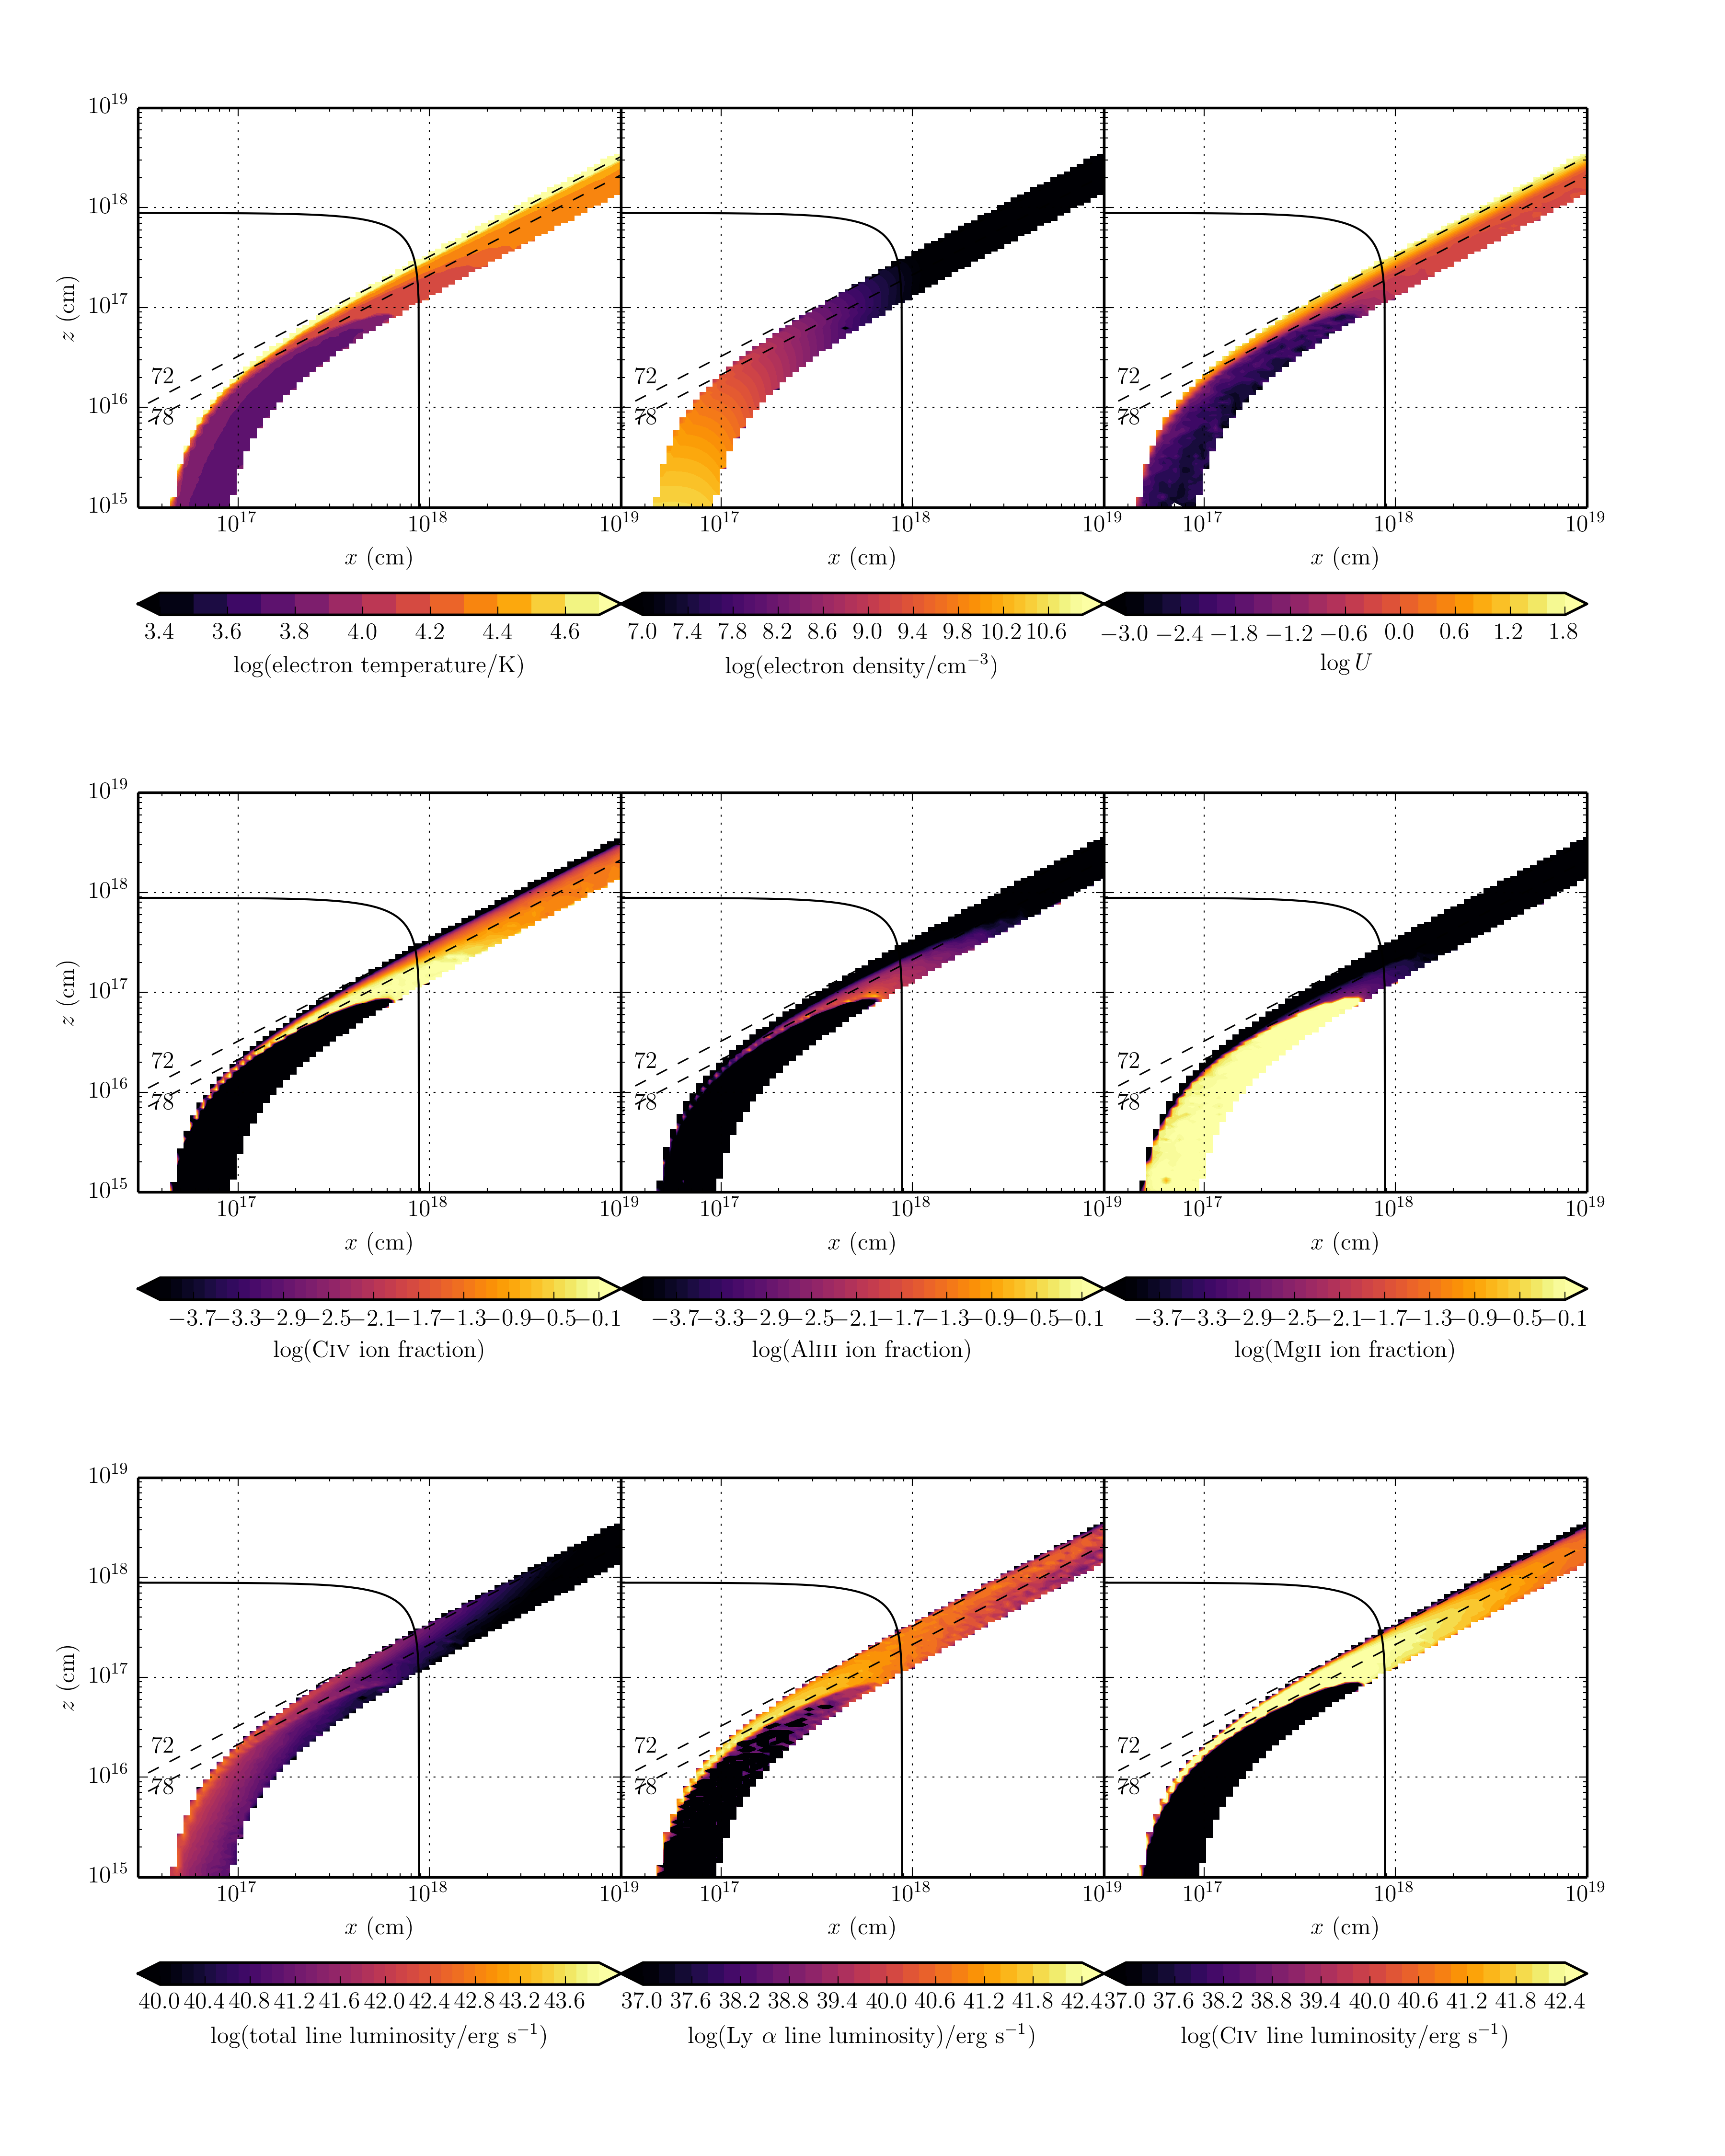
\includegraphics[width=1.0\textwidth]{figures/wind.png}
\caption
{
Physical properties of the outflow, shown by the coloured contours.
The solid black line marks a sphere at $1000~R_G$.
The dotted lines show the $72^\circ$ and $78^\circ$ sightlines 
to the centre of the system, and illustrate that different sightlines
intersect material of different ionization states.
}
\label{fig:uvspec}
\end{figure*} %fullpage

\begin{figure}
\centering
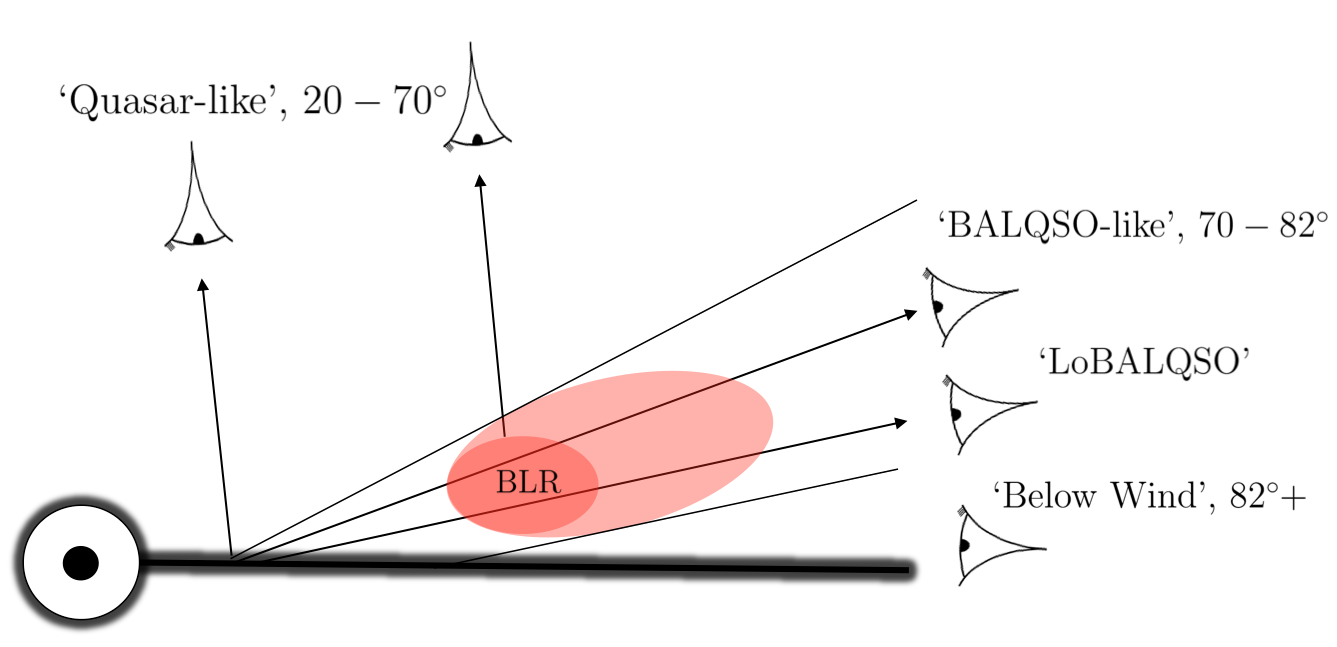
\includegraphics[width=0.5\textwidth]{figures/sightlines.png}
\caption
{
The classes of sightlines and the corresponding possible 
system types in the framework of our model.
%[FIGURE NEEDS IMPROVING]
}
\label{fig:lobal}
\end{figure}




\begin{table}
\begin{tabular}{p{3cm}p{4cm}}
\hline Free Parameters 	&	 Value \\ 
\hline \hline 
$M_{BH}$ 	 &	 $1\times 10^9~\rm{M_{\odot}}$ \\ 
$\dot{M}_{acc}$ 	 &	 $5~M_{\odot}yr^{-1} \simeq 0.2~\dot{M}_{Edd}$\\ 
$\alpha_X$ 	 &	 $-0.9$ \\ 
$L_{X} $ 	 &	 $10^{45}~\rm{ergs~s^{-1}}$$^*$ \\ 
$r_{disc}(min)=r_{X}$   &	 $6r_g=8.8\times10^{14}~{\rm cm}$ \\ 
$r_{disc}(max)$   &	 $3400r_g = 5\times10^{17}~{\rm cm}$ \\ 
$\dot{M}_{wind}$  &	 $5~M_{\odot}yr^{-1}$ \\ 
$r_{min}$ 	&	 $300r_{g} = 4.4\times10^{16}~{\rm cm}$\\ 
$r_{max}$ 	&	 $600r_{g} = 8.8\times10^{16}~{\rm cm}$ \\ 
$\theta_{min}$ 	&	 $70.0^{\circ}$ \\ 
$\theta_{max}$ 	&	 $82.0^{\circ}$ \\ 
$\lambda$ 	&	 $0$ \\ 
$v_{\infty}(r_0)$ 	&	 $v_{esc}(r_0)$ \\ 
$R_v$  	        &	 $10^{19}$cm$^*$ \\ 
$\alpha$ 	&	 $0.6^*$ \\
$f$ 	&	 $0.01^*$  \\
\hline 
% Derived Parameters 	&	 Value \\ 
% \hline \hline
% $L_{\nu}(2500\mbox{\scriptsize{\AA}})$&	 $6.3\times10^{30}~\rm{ergs~s^{-1}~Hz^{-1}}$\\ 
% $L_{\nu}(2keV)$   &	 $1.2\times10^{25}~\rm{ergs~s^{-1}~Hz^{-1}}$\\ 
% $L_{bol}$ 	 &	 $2.4\times10^{46}~\rm{ergs~s^{-1}}$\\
% $M_{bol}$ 	 &	 -27.4\\ 
% $M_u$            &	 -26.2\\ 
%  $\alpha_{OX} $ 	 &	 -2.2\\ 
\end{tabular}
\caption{Wind geometry parameters used in the model.}
\label{wind_param}
\end{table}



\subsection{Physical Conditions and Ionization State}

The wind rises slowly from the disc at first, with clumped densities
of $n_H \sim 10^{11}~\rm{cm^{-3}}$ close to the disc plane.
The flow then accelerates over a scale length of $R_V=10^{19}~\rm{cm}$
up to a terminal velocity of around $3$ times the escape velocity 
($\sim10,000~\rm{km~s^{-1}}$). This gradual acceleration means that
the wind exhibits a stratified ionization structure, with low ionization material
in the base of the wind giving way to highly ionized plasma further out.
By clumping the wind, we are able to produce the range of ionization states observed
in wuasars and BALQSOs, while adopting a realistic $2-10$ keV X-ray luminosity
of $L_{X}=10^{45}~\rm{ergs~s^{-1}}$. Without clumping, this wind would be over-ionized 
to the extent that opacities in e.g., \civ\ would be entirely negligible (see H13).

One commonly used measure of the ionization state is the ionization parameter, $U$, given by
\begin{equation}
U = \frac{4\pi}{n_H c}\int_{13.6{\rm{eV}}}^{\infty}\frac{{J_{\nu}d\nu}}{h\nu}.
\end{equation}
\noindent where $\rm{n_H}$ is the local number density of H, and $\nu$ denotes photon 
frequency. The ionization parameter represents the ratio of the number density of 
ionizing photons to the local H density. It is however, a poor measure of the 
ionization state of the resonance species such as \civ\ as it encodes no information
about the shape of the SED. In this case the X-ray photons 
are dominant in the photoionization of the UV resonance line ions. 
This explains why a factor of 100 increase in X-ray luminosity requires
a clumping factor of 0.01, even though the value of U decreases by only a factor of $\sim10$ 
compared to H13. This is also the reason for significant Lyman edge photoabsorption
at the highest inclinations (see section 4.3).

Clumping also causes the total line luminosity to increase dramatically,
as recombination and collisional excitation are both proportional to
$n_e^2$. This line emission typically emerges on the edge of the wind
nearest the central source. The location of the line emitting regions
is dependent on the ionization state, as well as the X-rays heating the plasma.
The radii of these emitting regions is important,
and can be compared to observations. Our \civ\ line emission region 
is located at about $1000~R_G$ ($\sim10^{18}~\rm{cm}$).
This is in rough agreement with the reverberation mapping 
results of Kaspi (2000) for the $2.6\times10^{9} M_\odot$ quasar S5 0836+71,
and also compares favourably with microlensing measurements of the size of the
\civ\ emission line region in the BALQSO H1413+117 \citep{odowd2015}.


\subsection{Synthetic Spectra}

\begin{figure*} %fullpage
\centering
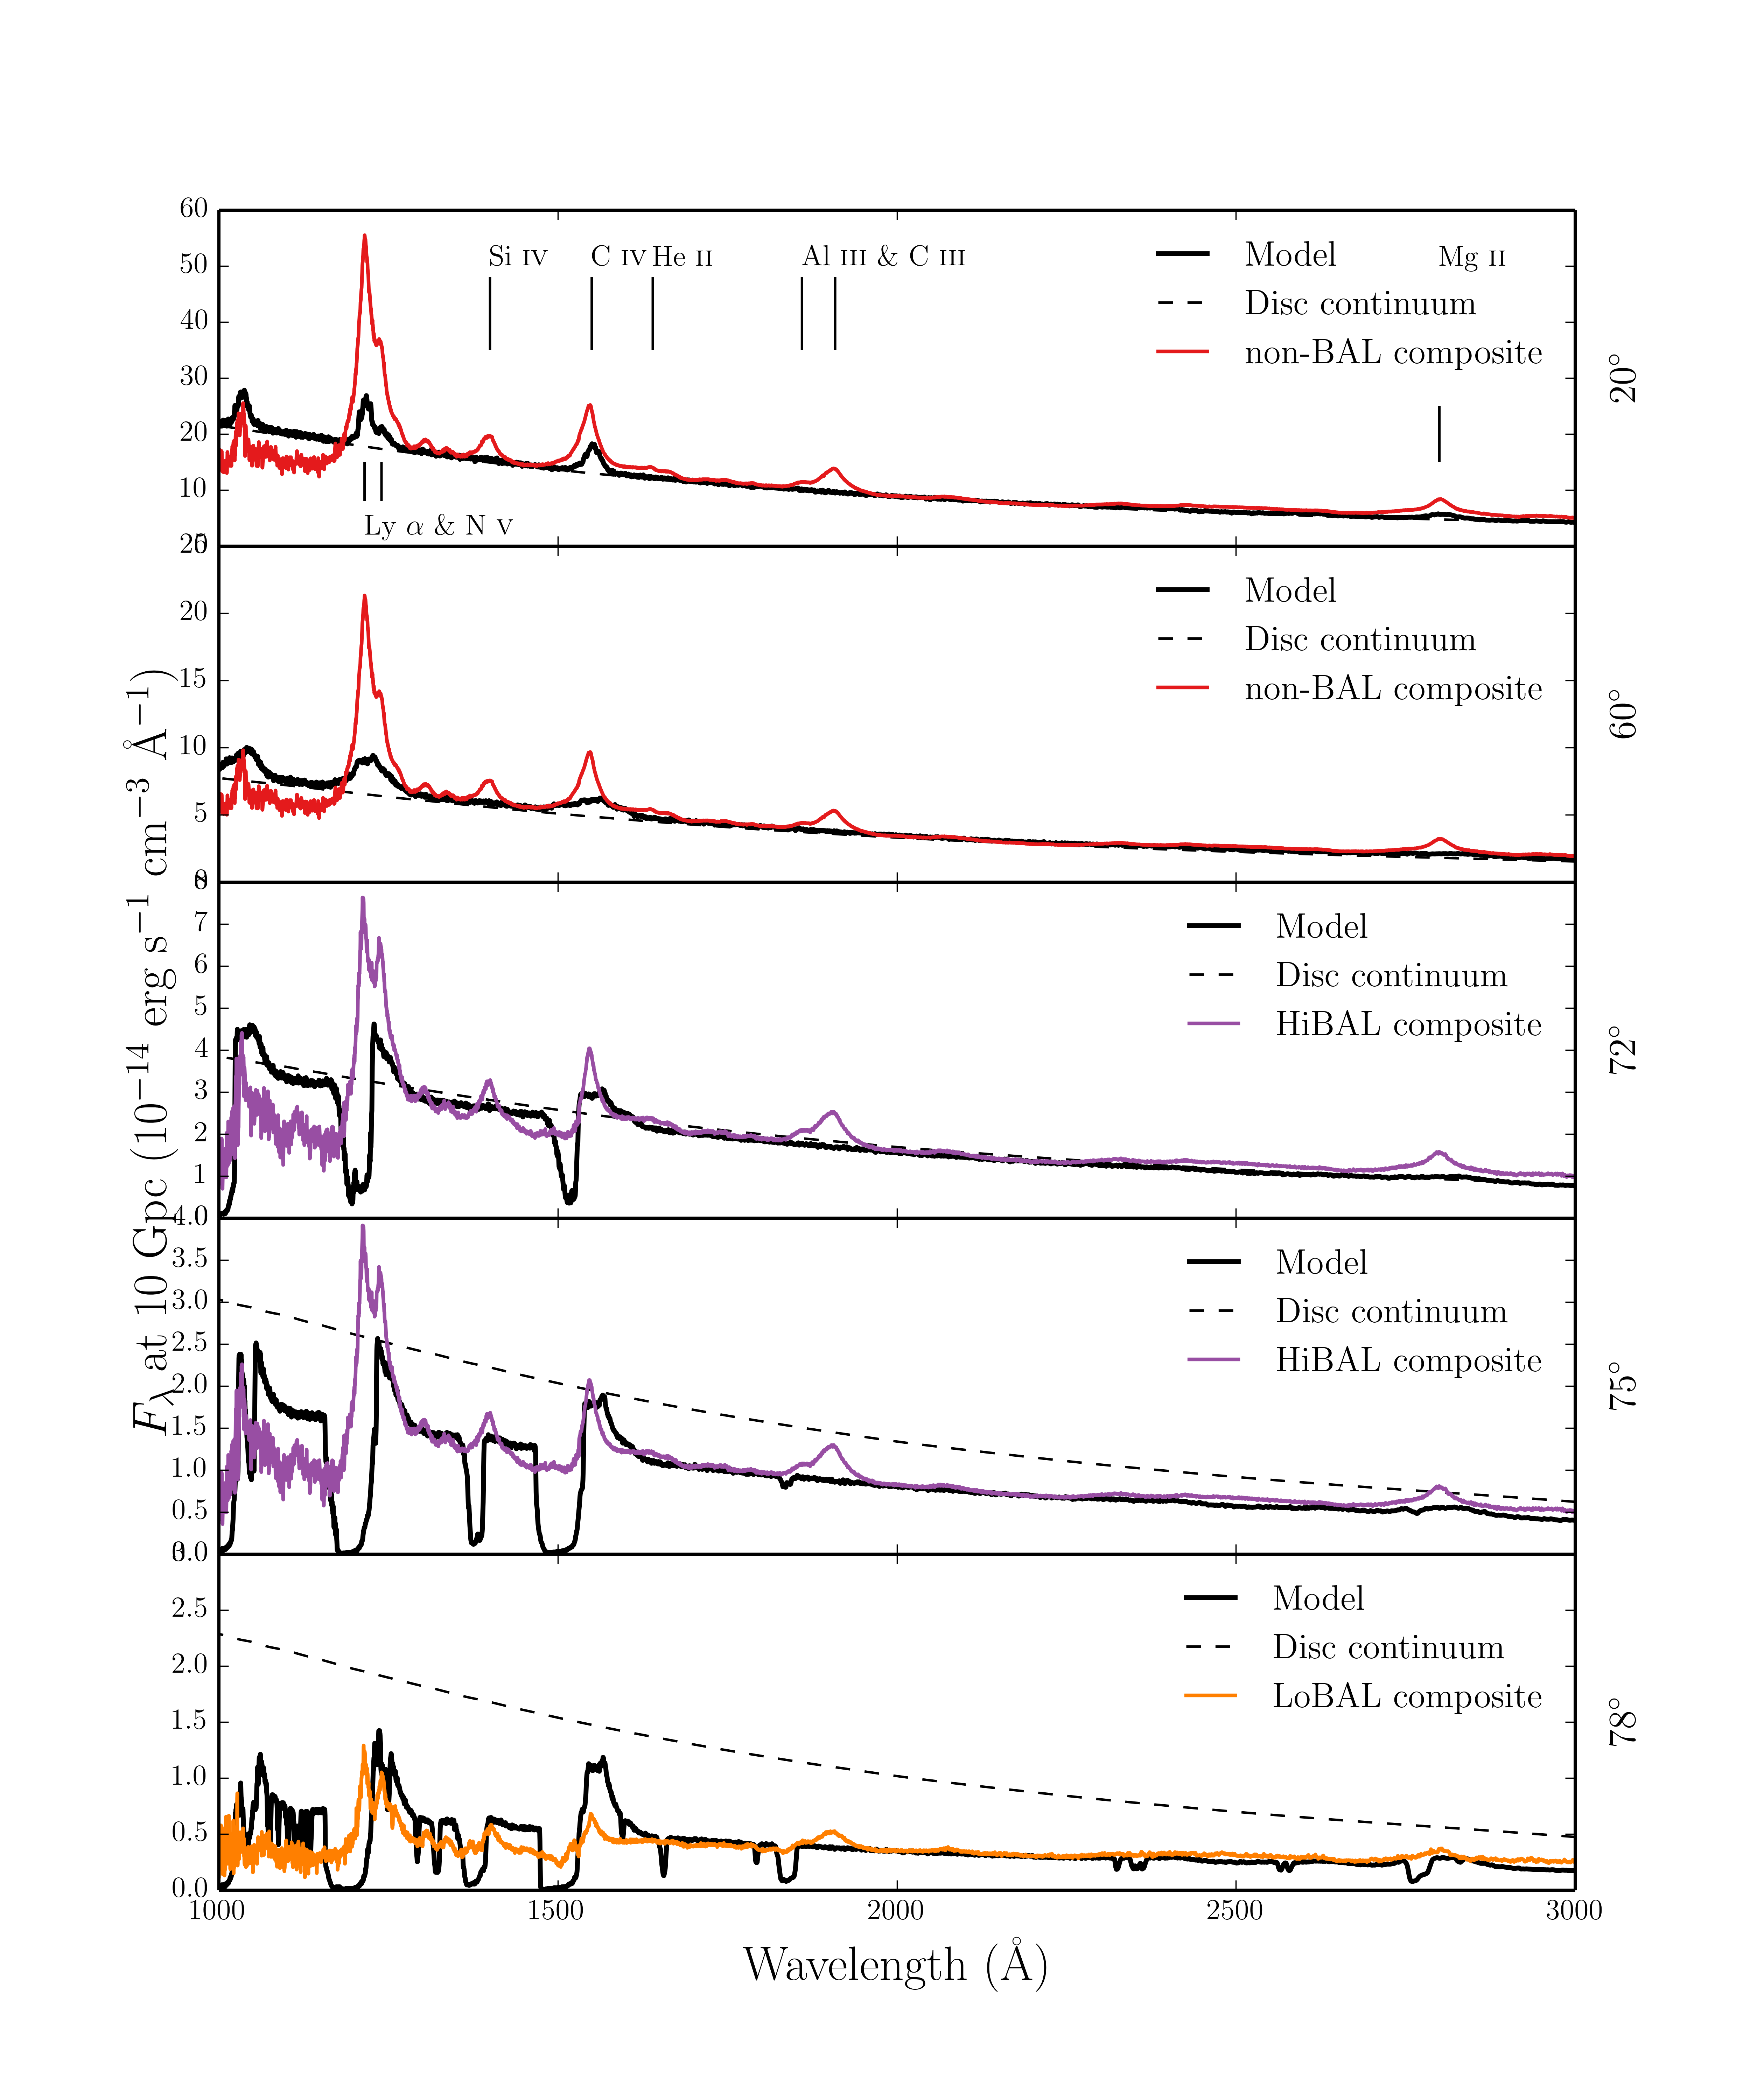
\includegraphics[width=1.0\textwidth]{figures/uvspec.png}
\caption
{
Synthetic spectra at four viewing angles in the clumpy model. Plot would look different probably,
and may show composites, but this would be the main synthetic spectrum plot.
}
\label{fig:uvspec}
\end{figure*} %fullpage

% \begin{figure*} %fullpage
% \centering
% 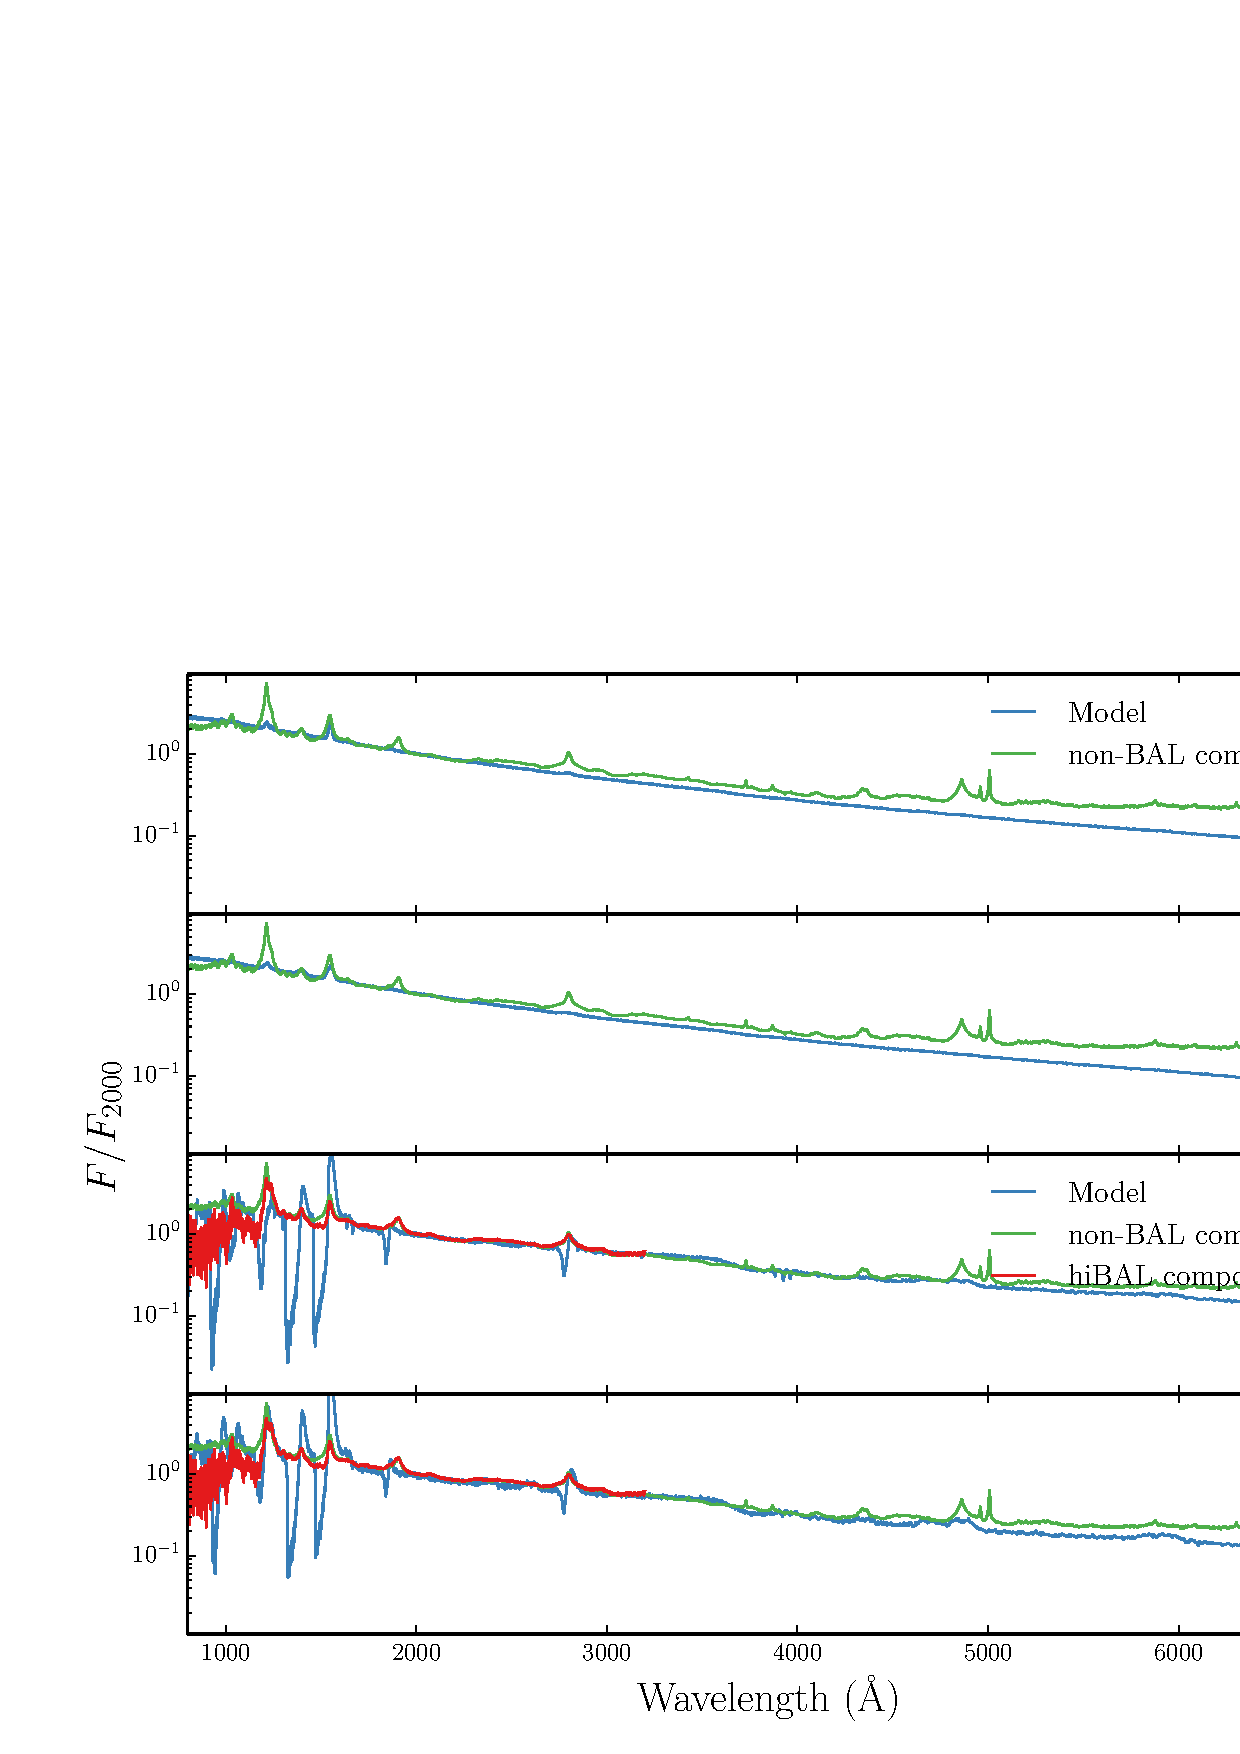
\includegraphics[width=1.0\textwidth]{figures/opt.png}
% \caption
% {
% Figure designed to show optical spectrum and comparison to composite.
% }
% \label{fig:uvspec}
% \end{figure*} %fullpage



Figure 4 shows the synthetic spectrum in the UV from the two models, with the
benchmark model from H13 also shown for comparison. We also show a comparison
to composite quasar and BALQSO spectra in figure 5, with the optical waveband 
included. In the UV, strong BAL profiles are formed in both models. This
highlights the first success of our model: clumping allows the correct ionization state 
to be maintained in the presence of strong X-rays. 
The BAL profiles are often saturated, and the location in velocity space
of the strongest absorption in the profile varies with inclination.
At lower inclinations, the strongest absorption occurs at the red edge,
whereas at high inclinations (and for the strongest BALs)
the trough has a sharp edge at the terminal velocity.
This offers one potential explanation for the wide range of BALQSO absorption
line shapes (see e.g. Trump et al. 2006; Knigge et al 2008).
In addition, the line profile shape is strongly dependent 
on the density, ionization and velocity 
profiles intersected by the line of sight. Thus, small tweaks of the velocity
law and angular distributions of streamlines can dramatically alter
the shape of the line.
% the line profile shape. Figure ?? shows selection of line profiles 
% for different kinematic parameters to demonstrate this. 
% The degeneracy between parameters, and lack of available
% physical and observational constraints goes someway to showing why individual 
% fitting of line profile shapes with kinematic models is such a difficult
% exercise.

We find that the model can produce significant line emission
at low inclinations, particular in \civ, 
and the improved treatment of recombination results in a strong \la\
line. In the context of unification, this is a promising results, 
and shows that a biconical wind can produce significant 
emission at `quasar-like' angles.
However, the red wing of the BAL profiles 
is generally stronger than seen in BALQSO spectra and composites.
This is due to a combination of strong collisionally excited emission
and continuum attenuation. To illustrate the amount of 
continuum attenuation we also show the continuum from a disc-only model.
The line-to-continuum ratios at low inclinations are also
significantly affected by disc foreshortening and limb darkening.
The angular distribution of the disc radiation is clearly
crucially important in determining the emergent line equivalent widths 
(EWs) -- this is discussed further in section~5.

To assess the ability of the model to match real 
quasar spectra, we also show {\sl Sloan Digital Sky Survey} (SDSS) quasar composites from
\cite{reichard2003}, normalised to the flux at 2000\AA\ in each panel.
The model matches the \civ\ and \mg\ line profiles fairly well, 
but the \la\ profile is a factor of $\sim3$ weaker than in the composite spectrum.
This is implies that a larger recombination line formation region is required in order 
to successfully reproduce the strong \la\ emission seen in 
all quasars. At the highest inclinations, the 
cooler, lower ionization material at the base of the wind
starts to intersect the line of sight. This produces 
multiple absorption lines lower ionization species such as \mg,
\al and Fe~\textsc{ii}, as well as strong Lyman continuum absorption.
The potential links to LoBALQSOs and FeLoBALQSOs are discussed in section 2.4.
% Figure 5 also shows the spectrum into the optical,
% showing that the outflow produces signiciant optical emission lines
% as well as having a noticeable effect on the continuum shape. This
% is particularly true around the Balmer jump at $3646\AA$ and is due to
% a prominent wind-formed recombination continuum.


\subsection{X-ray Properties and Broadband SEDs}

\begin{figure*} %fullpage
\centering
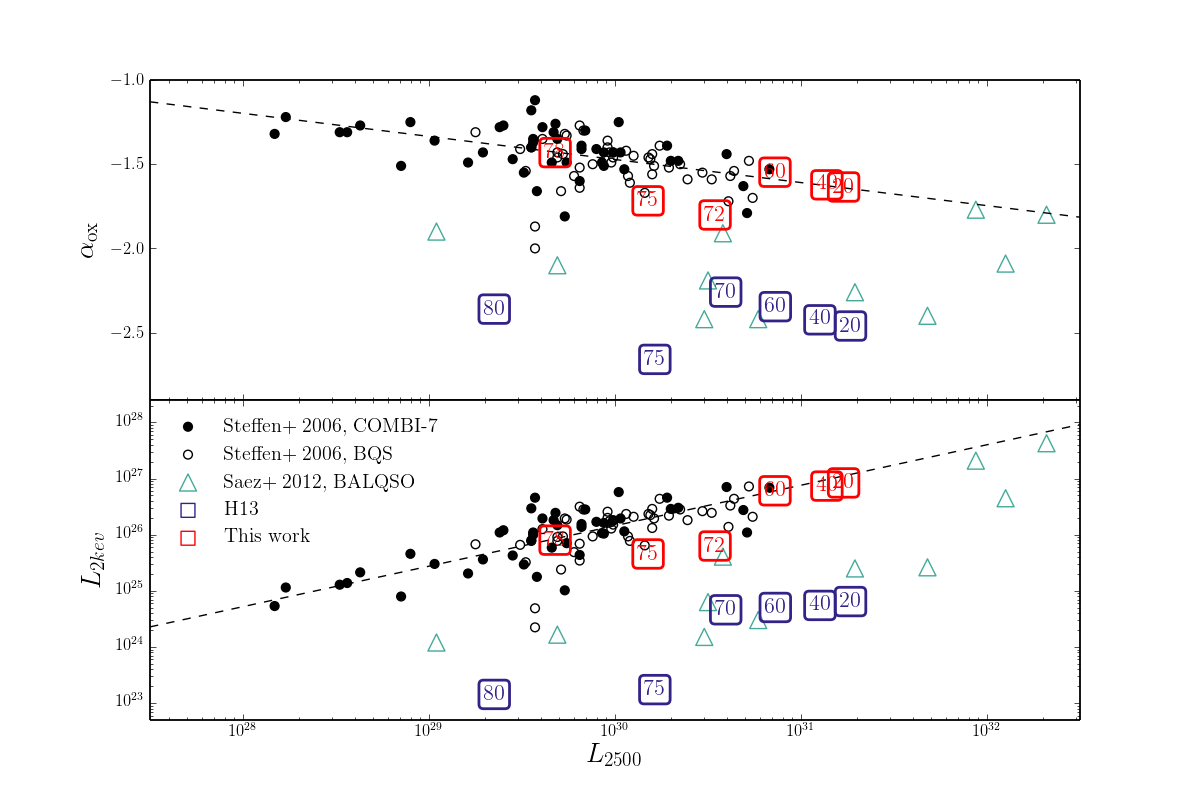
\includegraphics[width=1.0\textwidth]{figures/alpha_ox_both.png}
\caption
{
X-ray properties of the H13 and clumped model (text filled 
squares), plotted against monochromatic luminosity 
at 2500\AA. Also plotted are the samples considered by
Saez et al. 2012 on a similar plot; The COMBI-7 AGN and
the BQS samples Steffen et al. (2006) and the Saez et al. (2012) sample of BALQSOs.
The dotted lines show the best fit relations for non-BALQSOs from Steffen et al. (2006).
}
\label{fig:xray}
\end{figure*} %fullpage

% \begin{figure} %fullpage
% \centering
% 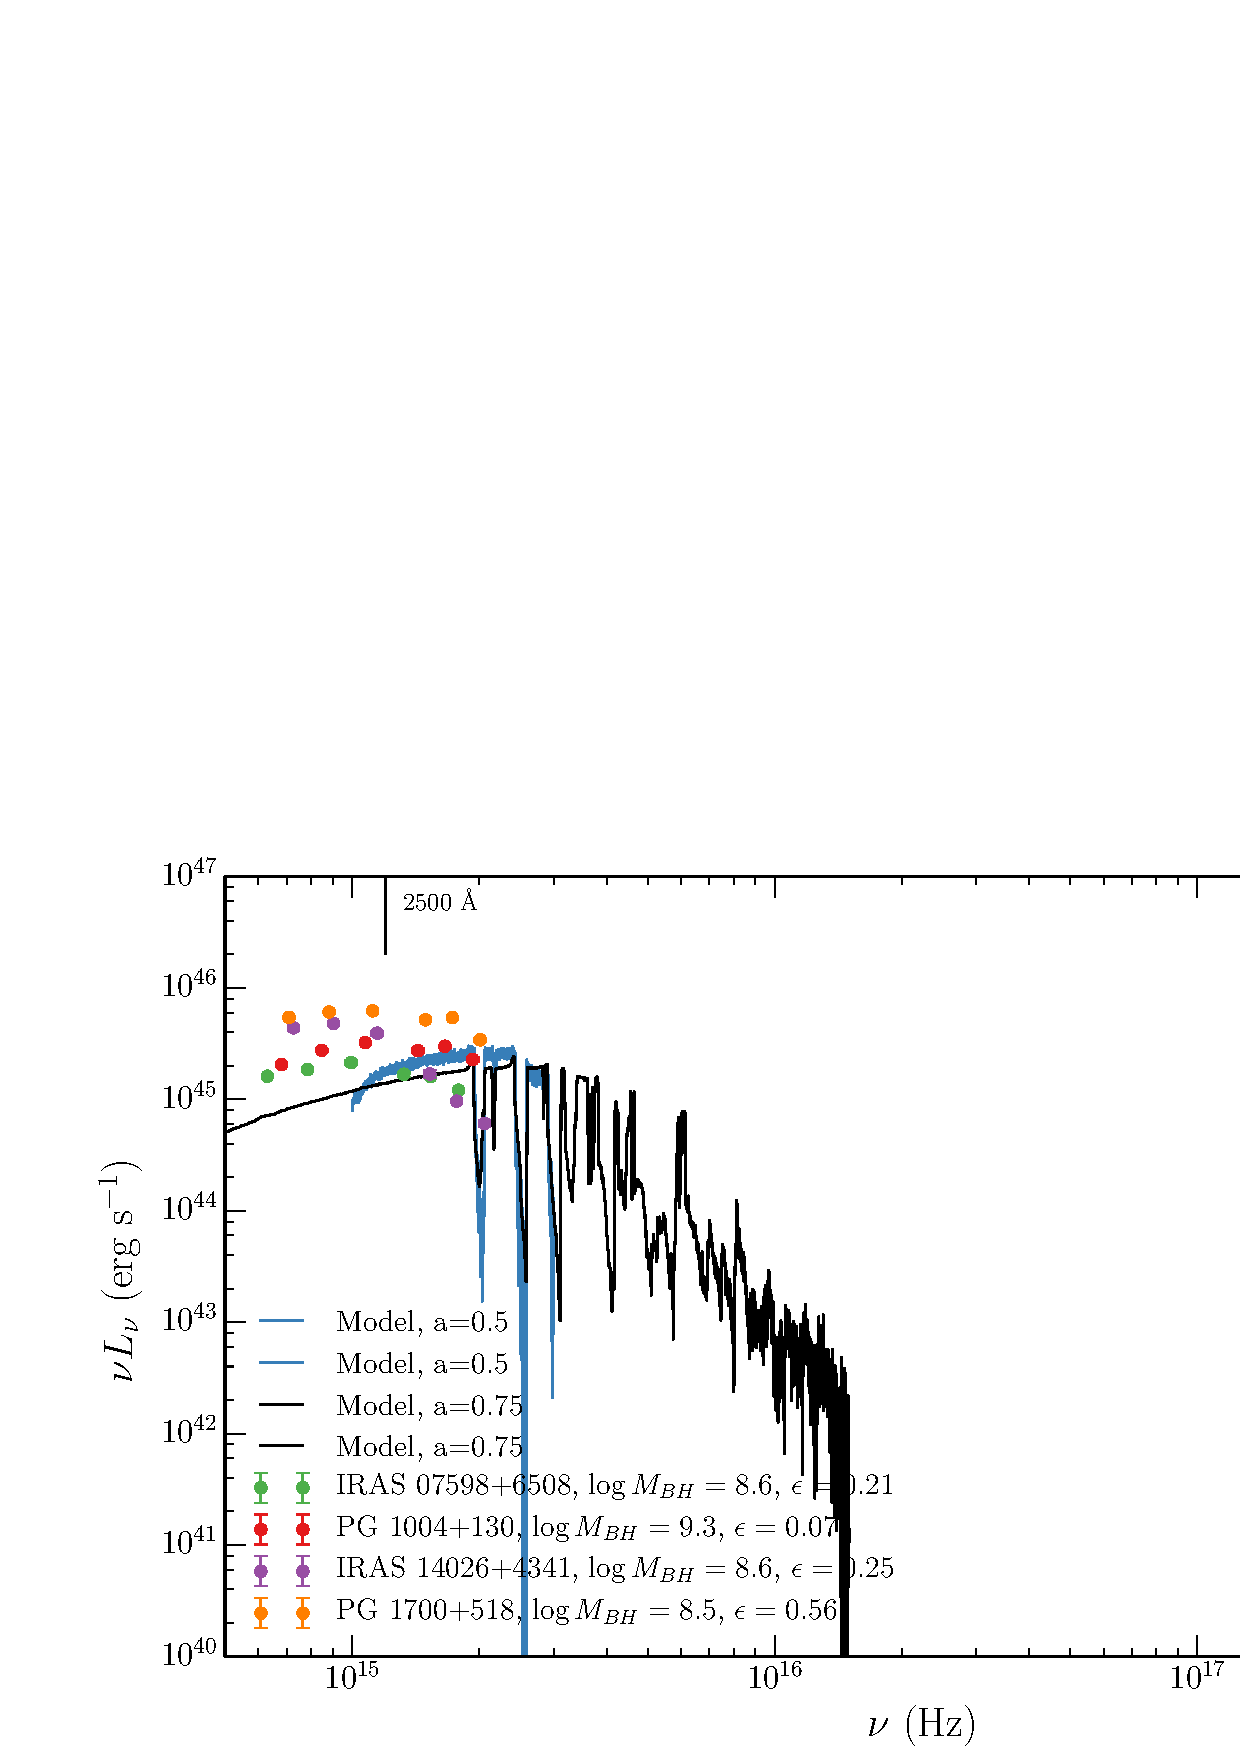
\includegraphics[width=1.0\textwidth]{figures/sed_all_balqsos.png}
% \caption
% {
% Broadband SEDs compared to IR and X-ray SEDs for selected BALQSOs 
% from Grupe \& Nousek (2015).
% }
% \label{fig:xray}
% \end{figure} %fullpage



Figure~\ref{fig:xray} shows the emergent
monochromatic luminosity ($L_\nu$) at 2~keV and $\alpha_{OX}$ plotted against 
$L_\nu$ at $2500$\AA\ for a number of different viewing angles in our model.
$\alpha_{OX}$ is a spectral index from near UV to X-rays defined by

\begin{equation}
\alpha_{OX}=0.3838\log\left(\frac{L_{\nu}(2~keV)}{L_{\nu}(2500~\mbox{\scriptsize{\AA}})}\right),
\end{equation}

which effectively represents a near-UV to X-ray flux ratio and a measure of X-ray 
weakness. The properties are calculated from the synthetic spectra and thus include
the effects of wind reprocessing and attenuation. In addition to model outputs,
we also show the BALQSO sample of Saez et al. (2012) and luminous AGN and quasar
samples from Steffen et al. (2006). The best fit relations from Steffen et al. (2006)
are also shown.
For low inclination, `quasar-like' viewing angles,
we now show excellent agreement with AGN samples. The trend with inclination
in our models is caused by a combination of disc foreshortening/limb-darkening 
(resulting in a lower $L_{2500}$ for higher inclinations) and the fact that the disk 
is opaque and thus the X-ray source subtends a smaller solid angle at high inclinations
(resulting in a lower $L_{2keV}$ for higher inclinations). 

Although the low inclination, `BALQSO-like' viewing angles show moderate agreement with the data,
it appears that our models tend to over-predict the emergent X-ray luminosity at BAL angles, 
although we are limited by poor statistics. 
% It is possible that this is due to our wind being overly optically thick to 
% electron scattering at angles which look through the wind. 
It could also be that the isotropic X-ray source assumption 
is incorrect and BALQSOs are {\em intrinsically} 
X-ray weak \citep[e.g.][]{morabito2013}. 
an anisotropic X-ray source might result in a lower clumping factor being
required in our model.
Nevertheless, our input X-ray spectrum
now reproduces the X-ray properties of a luminous quasar,
and at least some BAL angles match the .

Typically, BALQSOs show strong X-ray absorption with columns 
of $N_H\sim10^{23}~\rm{cm^{-2}}$ 
\citep{green1996,mathur2000,green2001,grupemathur2003}.
This is often cited as evidence that the BAL outflow is shielded from
the X-ray source, especially as sources with strong X-ray absorption tend
to exhibit deep BAL troughs and high outflow velocities 
\citep{brandt2000,laorbrandt2002,gallagher2006}.
Our results tend to imply that a clumpy BAL outflow
itself can be responsible for the strong X-ray absorption, 
and supports Hamann et al.'s (2013) suggestion that 
this explains the weaker X-ray absorption in mini-BALs 
compared to BALQSOs.

% We can also examine the emergent X-ray spectra from our model. 
% Our code is not yet optimized for producing X-ray spectra, as we do not yet 
% include all lines and levels of e.g. Fe or macro-atom treatments of 
% higher order ions (cf. Sim et al. 2008, 2010). 
% However, the bound-free opacity sources are complete, and comparisons of the shape
% of the heavily absorbed spectra can be useful.
% Figure 6 shows the broadband SED from the model, compared to a number of BALQSO spectra
% from \cite{grupenousek2015} - note that lower mass and super-Eddington sources
% are excluded. 

% discuss the figure showing X-ray properties briefly. 
% Present an X-ray spectrum? compare to observations e.g. Giustini?

% {\bf Figures 5 and 6: $L_{2kev}$ v $L_{2500}$ plot and X-ray spectrum compared to Grupe and Nousek (broadband SED?)} 

\subsection{LoBALs and ionization stratification}

\begin{figure*} %fullpage
\centering
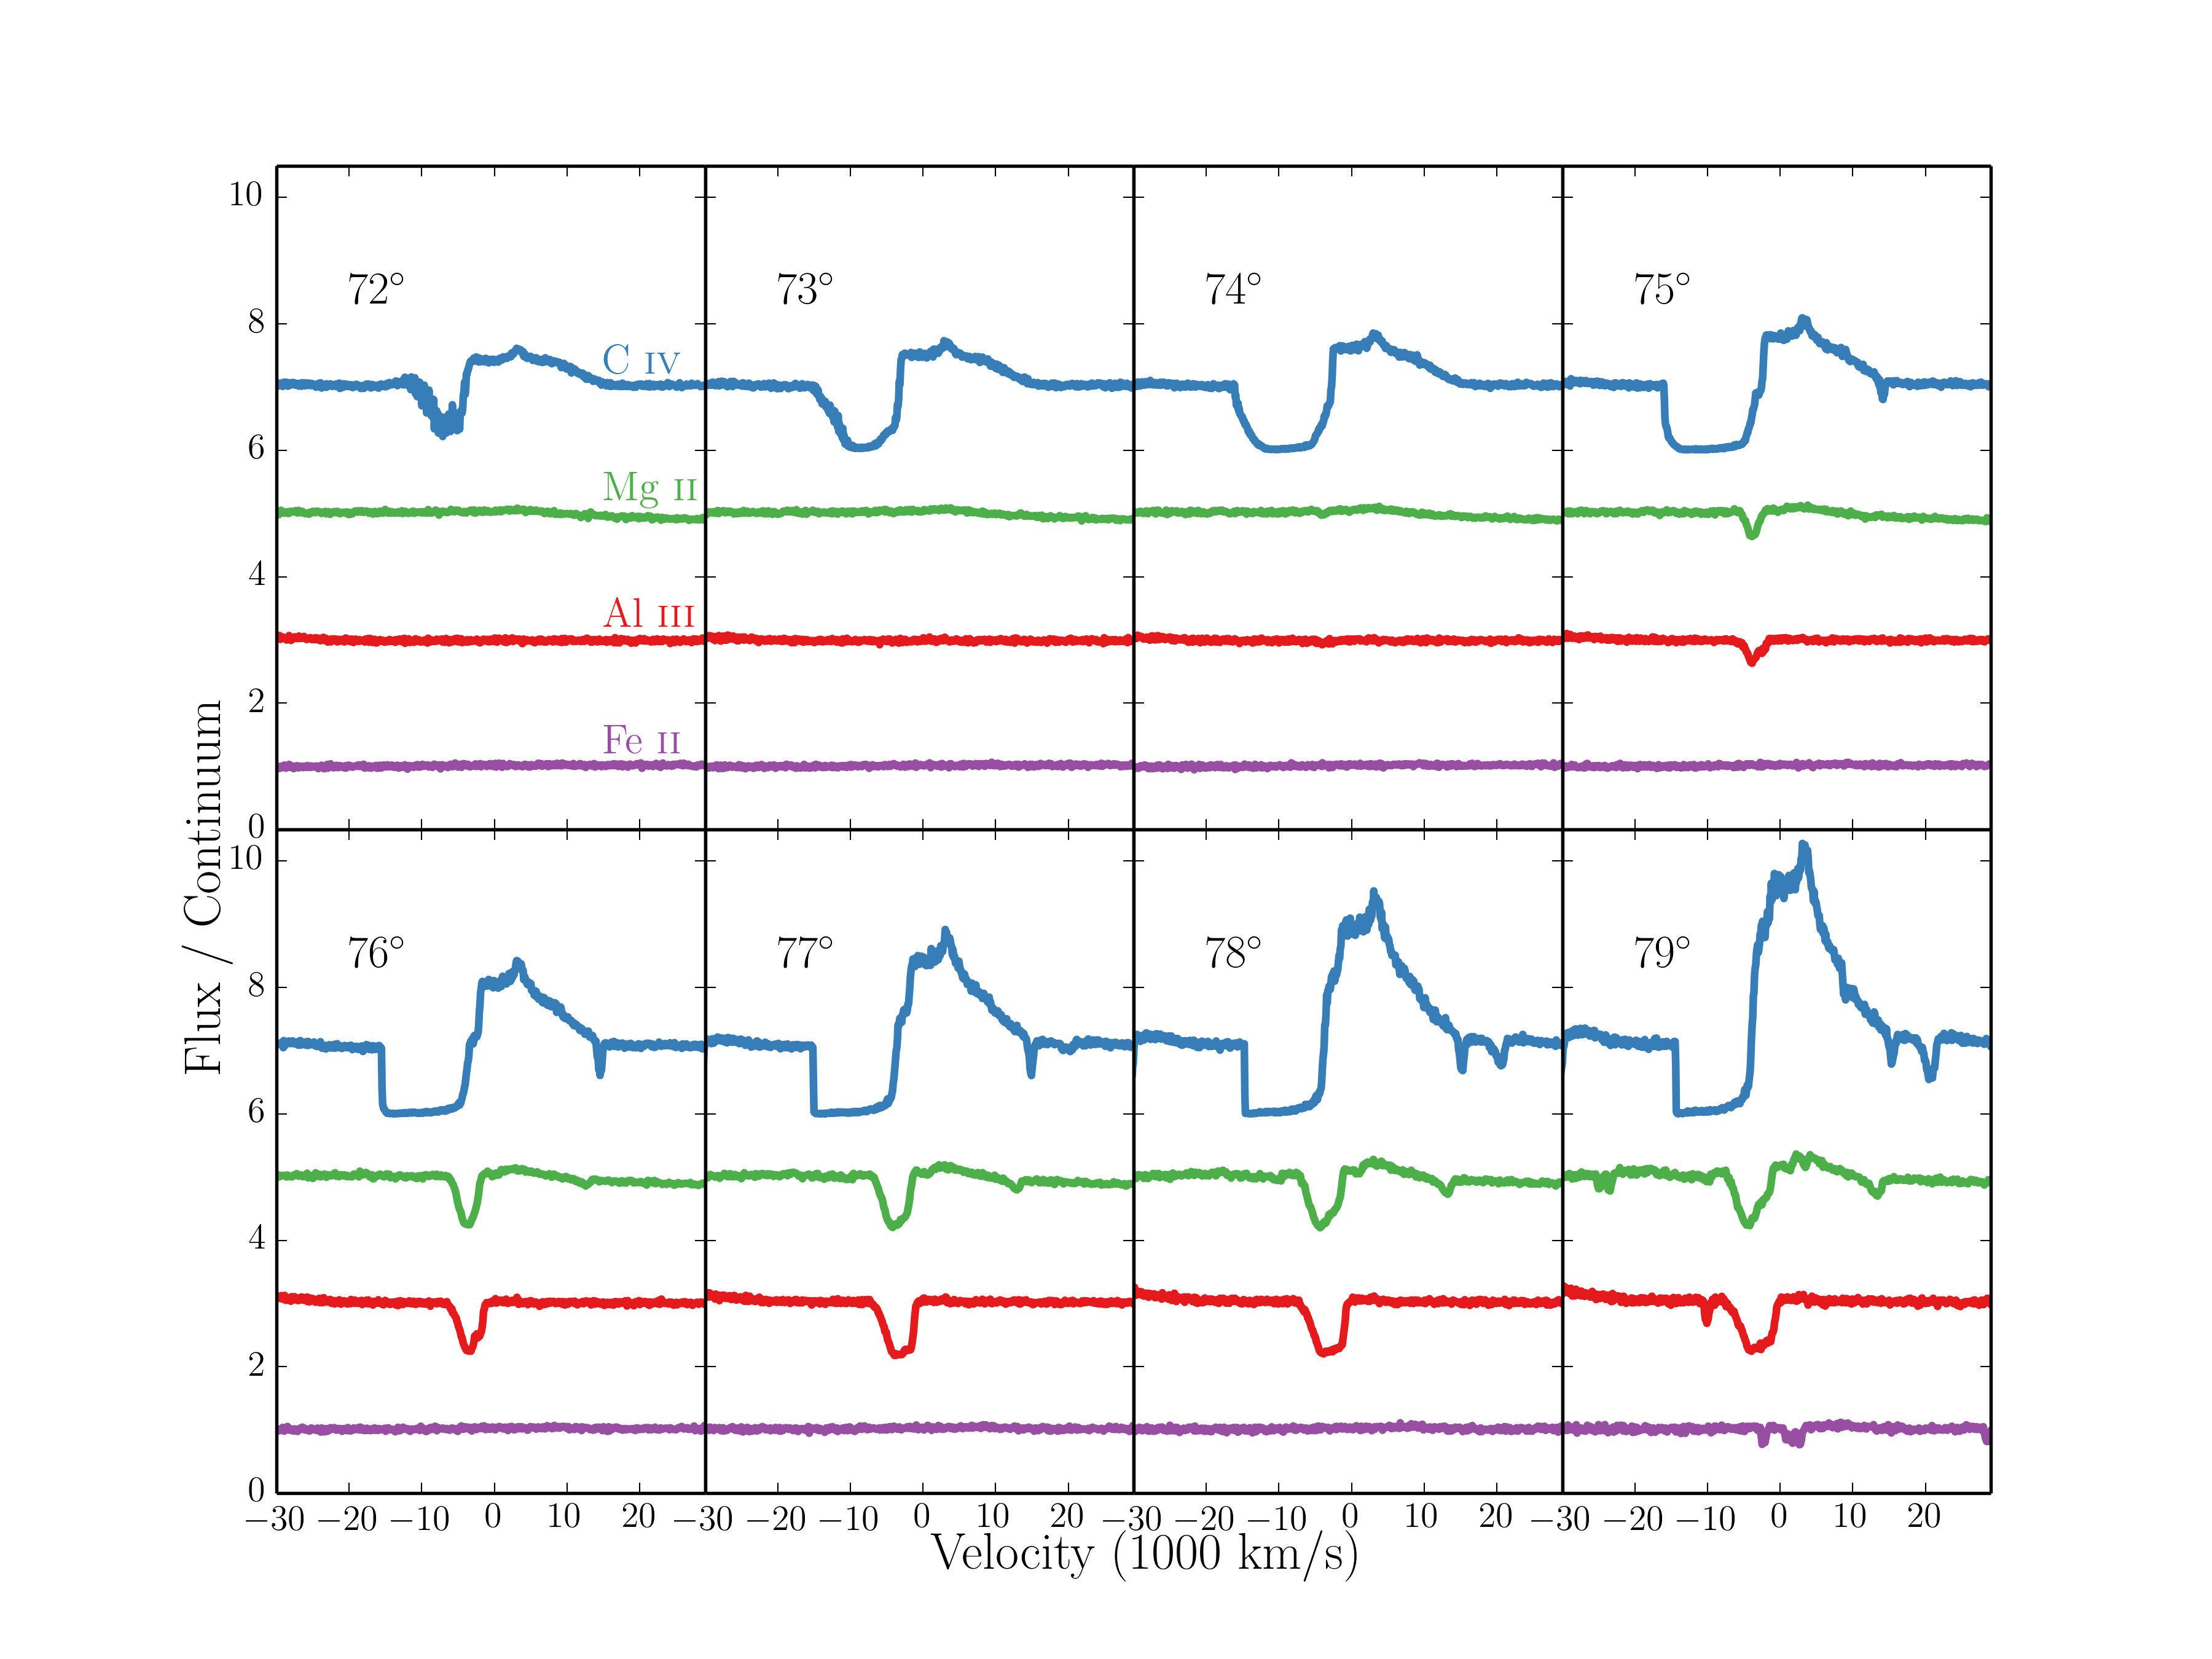
\includegraphics[width=1.0\textwidth]{figures/c4_angles.png}
\caption
{
\civ , \mg , \al\ and Fe~\textsc{ii} line profiles for wind angles
from $72-79^\circ$. The profiles are plotted relative to the local
continuum with an offset applied for clarity. Lower ionization
profiles appear at a subset of high inclinations, compared
to the ubiquitous \civ\ profile.
}
\label{fig:lobal}
\end{figure*} %fullpage


At certain sightlines, our model now produces blue-shifted BALs in \al\ and \mg --
the absorption lines seen in LoBALQSOs, and we even see absorption in Fe~\textsc{ii}
at the highest inclinations. Line profiles in velocity space 
for \civ, \al\ and \mg, are shown in figure~\ref{fig:lobal} for a range
of BALQSO viewing angles. We confirm the behaviour expected from 
a unification model such as Elvis (2000), in which ionization stratification
explains the incidence of LoBALQSOs. We find, that the lower
ionization material is intercepted by a smaller family of sightlines as shown by 
figures~\ref{fig:wind} and \ref{fig:lobal}.
There is also a correlation between the strength of LoBAL features
and the amount of continuum attenuation at that sightline. 
This offers a potential explanation for the rarity of LoBAL and
FeLoBAL quasars (but see also section~\ref{sec:balfrac}).

% These line profiles also indicate a potential problem with our model. 
% \cite{odowd2015} find that the LoBAL profiles in H1413+117 have a 
% higher velocity onset than the higher ionization BALs, suggesting that the
% wind becomes less ionized as radius increases. 
% We find the opposite trend in velocity onsets. In addition, examination of 
% figure~\ref{fig:wind} shows that ionization parameter decreases with radius, 
% because the decrease in density wins over geometric dilution of the radiation 
% field. While the \cite{odowd2015} hypothesis comes from one object,
% it is clear that {\em at least some} BALQSOs must become less ionized at 
% higher velocities, contrary to what one expects from our modelling.





%%%%%%%%%%%%%%%%%%%%%%%%%%%%%%%%%%%%%%%%%%%%%%%%%

% DISCUSSION 

%%%%%%%%%%%%%%%%%%%%%%%%%%%%%%%%%%%%%%%%%%%%%%%%%

\section{Discussion: The Disc SED}

When comparing BALQSO and quasar composites, it is apparent
that they possess remarkably similar line strengths and widths 
\citep[e.g.][]{reichard2003}.
This presents a challenge to our model, as well as the geometric 
unification picture in general.
Limb darkening and foreshortening causes the disc continuum emission to be 
strongly anisotropic. Coupled with attenuation from the wind, 
this has the effect of enhancing the 
line-to-continuum ratios at high inclinations, to the extent
that the \civ\ line can have an equivalent widths of ?? at $80^\circ$
compared to ?? at $20^\circ$. To construct a scenario where emission 
line equivalent widths are comparable at all inclinations requires 
significant fine-tuning when considering a classical thin disc. 
An alternative, simpler solution is that the emergent continuum is roughly isotropic.
This could potentially be achieved by wind reprocessing or a more realistic, GR treatment
of the accretion disc. We briefly discuss both these possibilities.

\subsection{Wind reprocessing}

If the majority of continuum radiation was reprocessed by nearby photoionized plasma (such 
as the outflow itself), then this would result in a roughly
isotropic radiation field. There are a number of appealing aspects to this scenario.
First, it may go some way to explaining recent microlensing (REFs) and timing (REFs)
observations which suggest that accretion disc sizes are a factor of $\sim3$ 
larger than one expects from a Shakura \& Sunyaev (1973) thin disc. 
Second, it implies a wide angle, large covering factor wind in order to 
intercept most of the disc continuum. This would make the outflow 
an effective feedback mechanism \citep[e.g.][]{borguet2012}, 
and would imply that BALQSO outflows
have a similar geometry to the ultra-fast outflows seen in nearby AGN 
\citep[e.g.][]{reeves2003,poundsreeves2009,tombesi2010a}.
We note that spectropolarimetry of BALQSOs shows that the light from BAL troughs is $\sim10\%$ 
linearly polarised, but the continuum generally has negligible polarisation \citep{lamy2000}.
This suggests that the continuum of BALQSOs cannot be significantly enhanced by
{\em single} scattering into the line of sight, but does not rule out 
{\em multiple} scatterings leading to a more isotropic continuum. 

\subsection{General relativistic effects}

General relativistic effects -- specifically, light bending
and relativistic beaming -- can cause 
the accretion disc SED to become more isotropic \citep[e.g.][]{zhang1997,munozdarias2013}.
To generate GR disc spectra, we use the code \agn\ \citep{hubeny2000,davishubeny2006,davis2007}. 
The output flux at three different wavelengths
as a function of inclination for an \agn\ model with the same disc and BH parameters
as our clumpy wind model is shown in figure~\ref{fig:f2000}.
The effects of GR on an AGN disc are much less extreme 
in the UV portion of the spectrum than the calculations
by \cite{zhang1997} for the X-rays in X-ray binaries.
As a result, the disc emission is still strongly anisotropic.
GR alone therefore cannot explain the line ratio trends in quasars.

% To examine the effect of GR on our models, we carry out the following procedure.
% First, we fit our output spectrum with a polynomial. This continuum fit can 
% be subtracted from the actual spectrum 
% to produce a model of the line emission only. We then calculate the 
% `wind continuum factor', by comparing the model fit with the emergent 
% disc spectrum without a wind. This factor gives us an approximate way to quantify the 
% effect of the wind on a disc continuum. It will generally be $>1$ at high inclinations,
% and $<1$ at low inclinations. This calculates emergent accretion disc spectra from an AGN disc atmosphere
% including relativistic effects. Finally, produce our final synthetic spectrum 
% by convolving this the line emission spectrum with the \agn\ model for the model parameters.

% Figure 10 shows the resultant spectrum. Including GR clearly helps


% Can GR effects offer a potential solution? (not quite!)

% {\bf Figures 8 and 9: AGNSPEC F(2000) as a function of viewing angle compared to a BB disc.
% spectrum compared to composites with AGNSPEC correction.} 

\begin{figure}
\centering
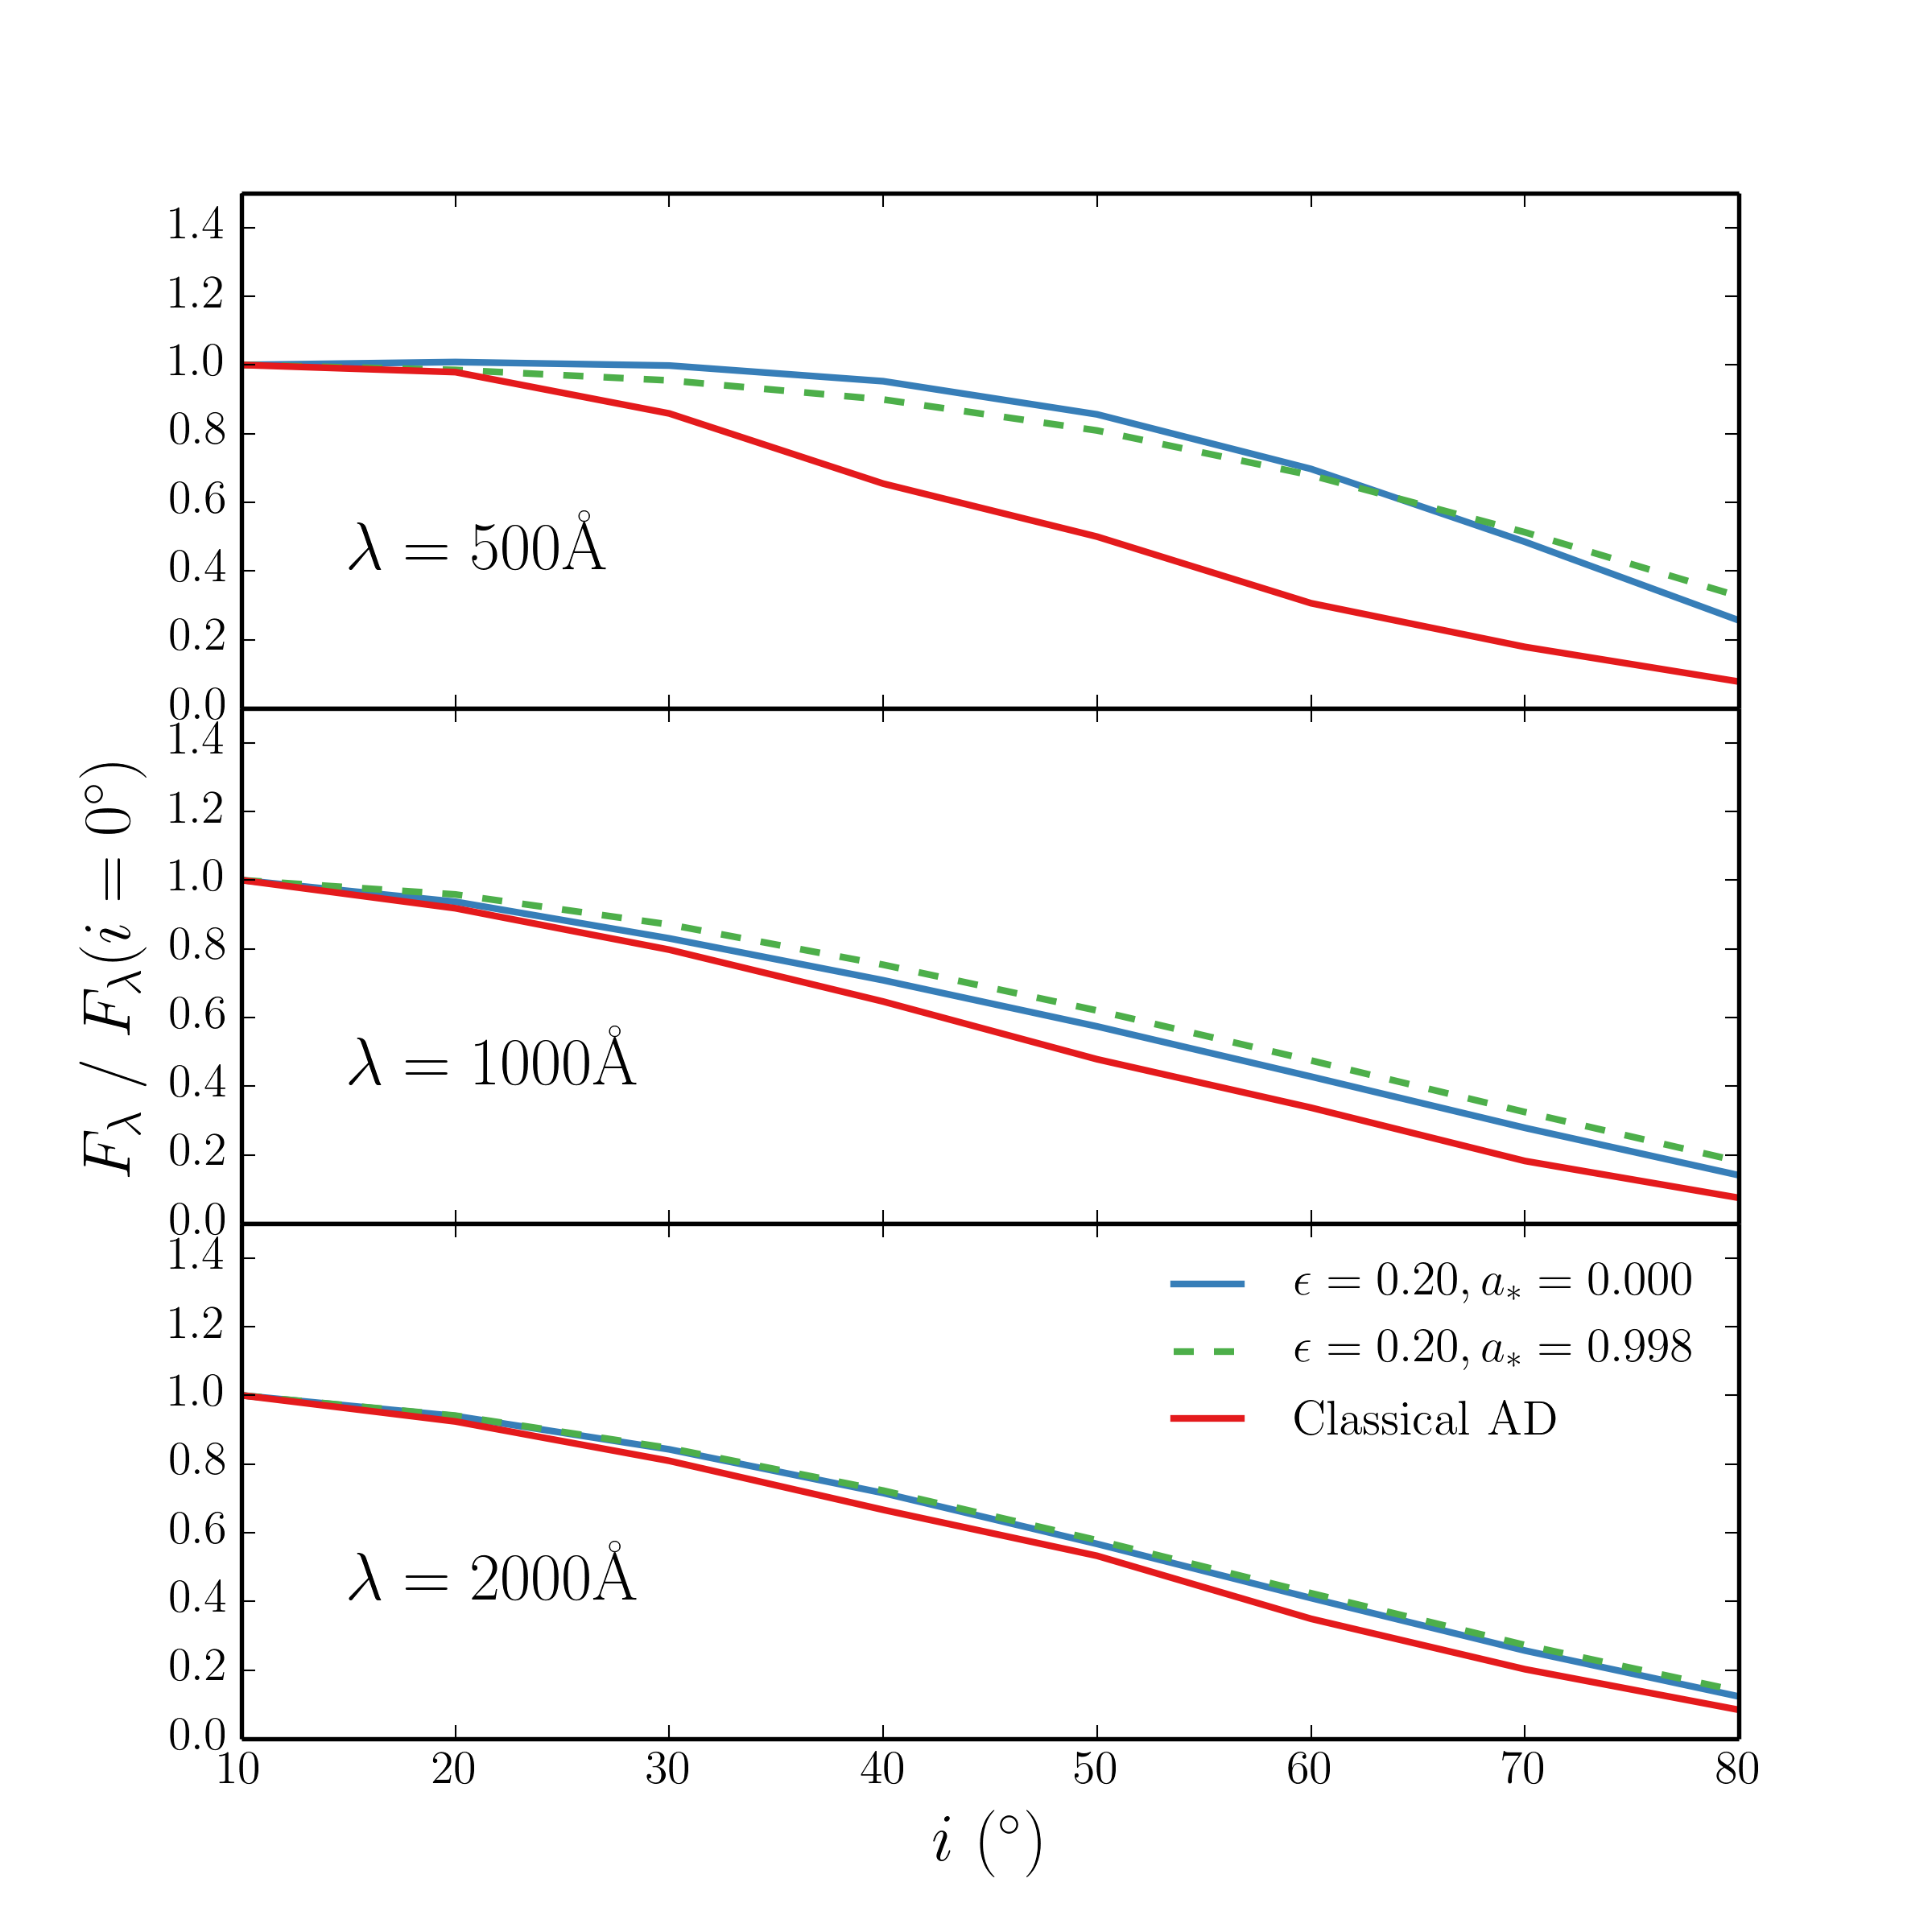
\includegraphics[width=0.5\textwidth]{figures/agnspec.png}
\caption
{
$F_\lambda$ for three different wavelengths
as a function of inclination from \agn\ models, 
compared to a classical AD. 
The \agn\ models are computed for Kerr and Scharzschild
BHs with the same $M_{BH}$ and $\dot{m}$ as our model.
}
\label{fig:f2000}
\end{figure}

% \begin{figure*} %fullpage
% \centering
% 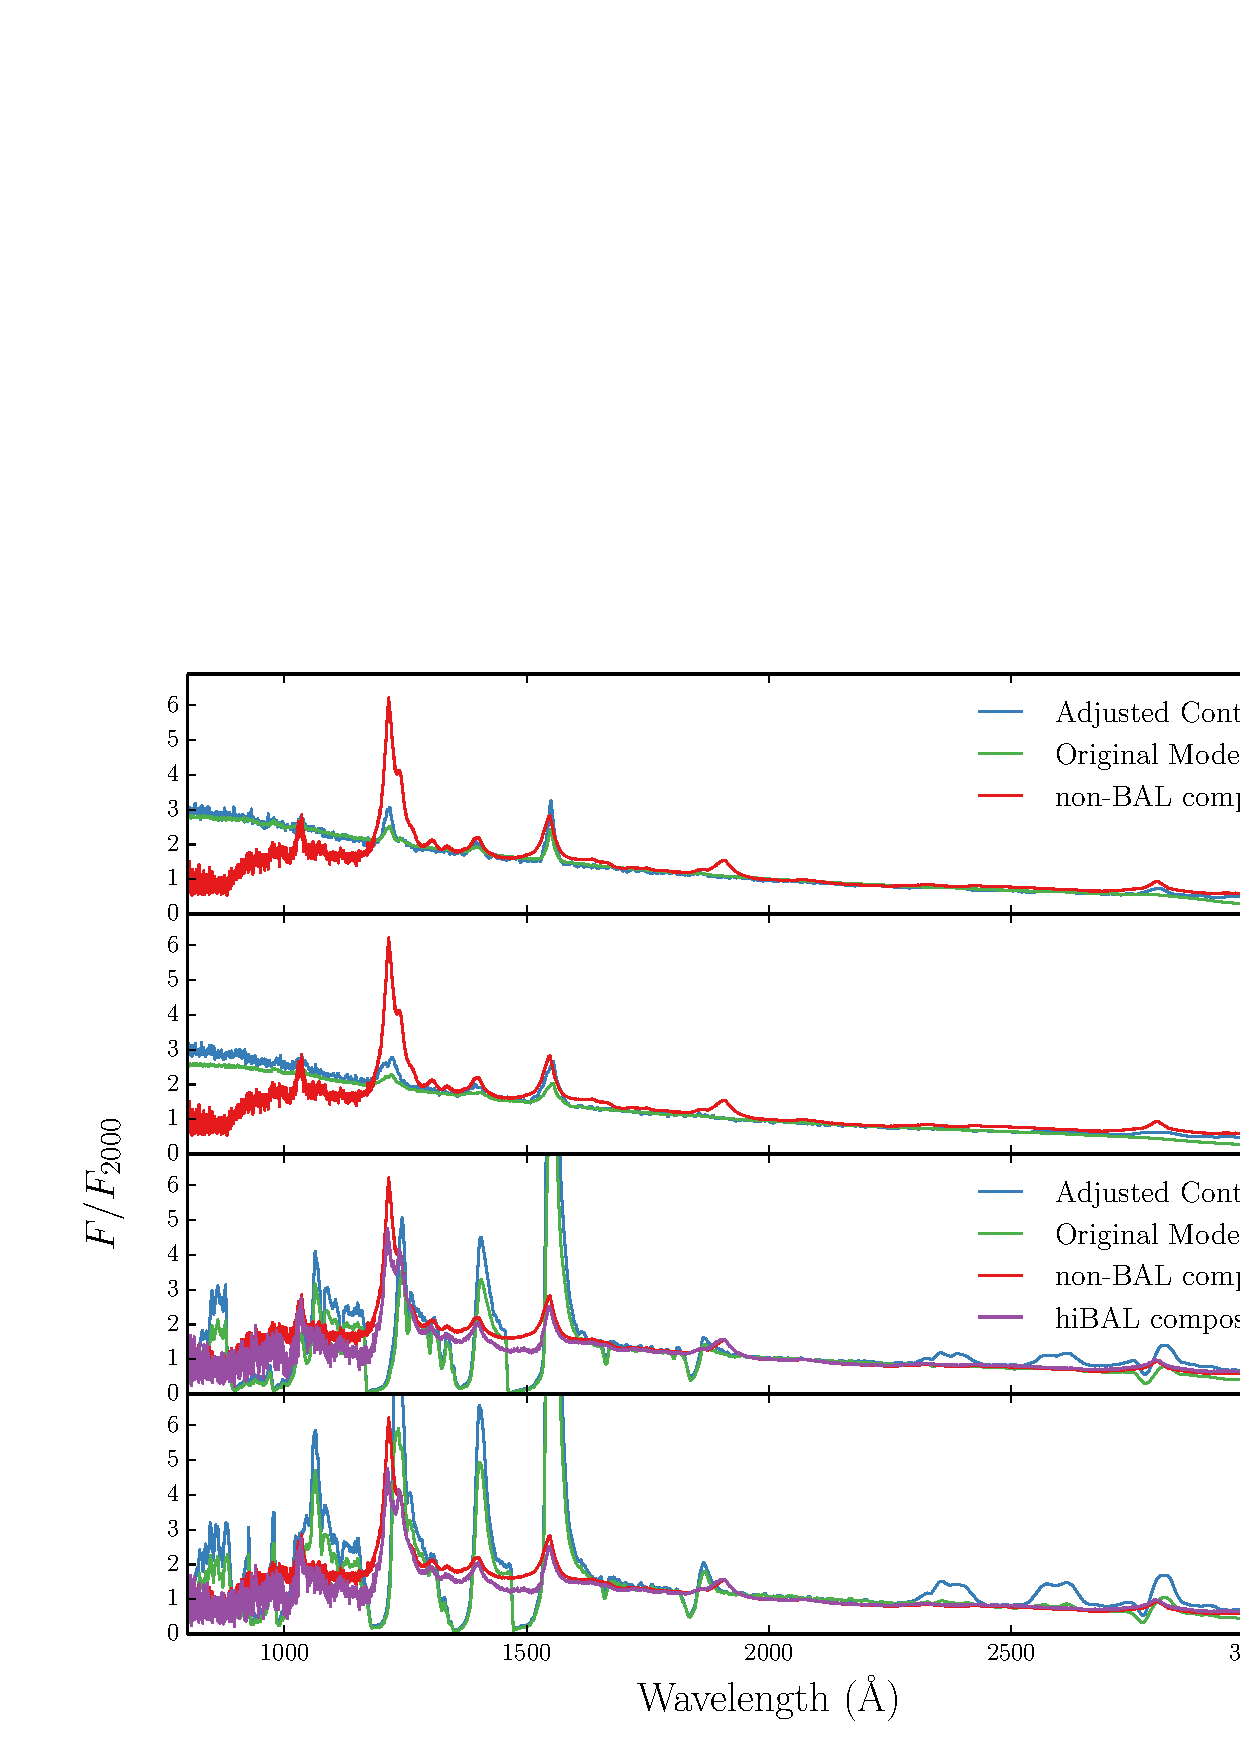
\includegraphics[width=1.0\textwidth]{figures/adjusted_withbals.png}
% \caption
% {
% $F_\lambda$ normalised to $F_{2000}$. {\bf Again, this is a placeholder- but I'm thinking some kind of comparison to composite including the adjusted continuum, showing that we can't get it exactly right}.
% }
% \label{fig:finalcomp}
% \end{figure*} %fullpage





\subsection{The BALQSO fraction and wind covering factor}
\label{sec:balfrac}

The disc SED has a profound effect on the intrinsic BAL fraction
inferred from flux-limited samples. This in turn impacts on 
the geometry and covering factor assumed for BALQSO and unified wind models,
and even effects the efficiency of feedback.
\cite{krolik1998} noted that the effect of limb darkening and foreshortening
would result in a signicantly underestimated covering factor for BALQSO winds.
The effect is complicated further by the quasar luminosity function -- if 
BALQSOs have lower observed luminosities for given accretion disc properties 
then they may be drawn from a different bin in the quasar luminosity function 
\citep{goodrich1997}. This will also have a similar impact
on the LoBALQSOs and FeLoBALQSOs sub-populations.
The complex (and as yet unknown) selection effects are understandably 
not taken into account by current estimates of the intrinsic BALQSO fraction 
\citep{weymann1991, reichard2003, knigge2008, turnermiller2009, allen2011}. 

The way forward is somewhat unclear. Given the lack of available observational 
constraints, models cannot readily be used to inform the selection criteria when 
calculating the BALQSO fraction. There are two main possibilities:
First, the disc emission is roughly isotropic, in which case the BAL fraction
estimates should be a good estimate of the covering factor of the outflow,
but the question about how this isotropy is achieved remains outstanding.
Or second, the disc emission is strongly anisotropic, which follows more
naturally from a disc geometry but has large implications
for the inferred covering factors, as well as leaving the similar line strengths
in BAL and non-BAL quasar compoosites unexplained (see previous sections).
Understanding the true nature of the disc SED, including the
angular distribution of radiation, is clearly crucial in order
to accurately estimate the true covering factor of BALQSO winds.

% A brief comment, citing Goodrich / Krolik \& Voit on the 
% way in which anisotropy / attenuation affect the inferred
% BAL fraction. We also need to be aware that there will be a number of selection
% effects in building up the composites, and we should discuss these
% and the subtleties involved. 

% \begin{figure}
% \centering
% 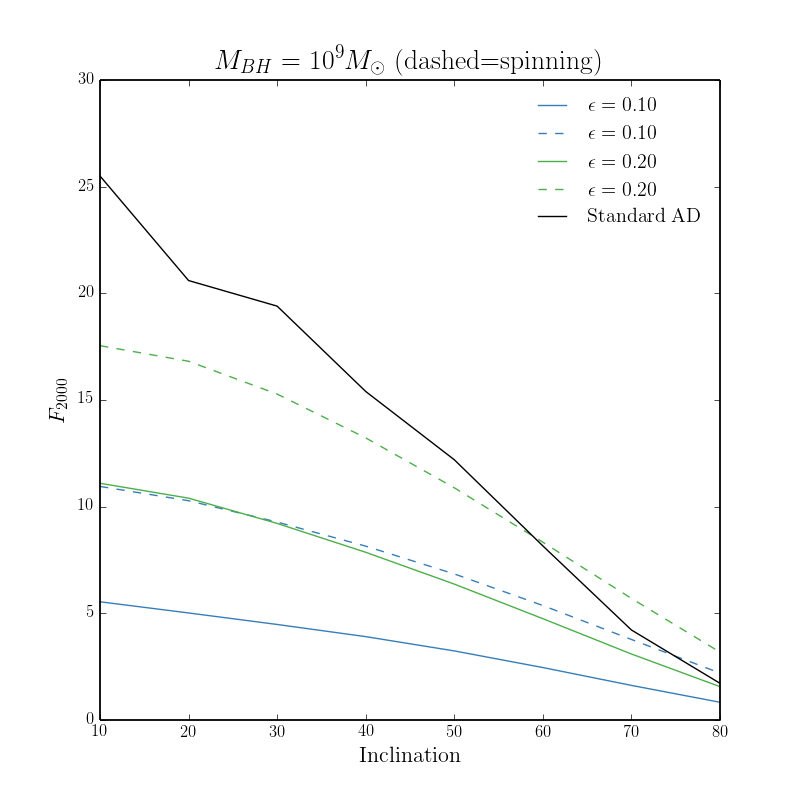
\includegraphics[width=0.45\textwidth]{figures/f2000_m9.png}
% \caption
% {
% $F_\lambda$ at $2000$~\AA\ as a function of inclination from
% \agn\ models. Spectra are computed for BH of $10^9~M_\odot$ with
% a number of different BH spins and Eddington fractions. The black line
% shows a standard multi-temperature blackbody AD model.
% }
% \label{fig:alpha_ox}
% \end{figure}




%%%%%%%%%%%%%%%%%%%%%%%%%%%%%%%%%%%%%%%%%%%%%%%%%

% SUMMARY

%%%%%%%%%%%%%%%%%%%%%%%%%%%%%%%%%%%%%%%%%%%%%%%%%

\section{Summary}

We have carried out MCRT simulations using a simple
prescription for a biconical disc wind, with
the aim of expanding on the work of H13 and assessing 
the viability of such a model for geometric unification of quasars.
We find the following main points:

\begin{enumerate}
\item We have introduced a first-order treatment 
of clumping in our model, and found that it can now maintain
the required ionization state while agreeing well with the X-ray
properties of AGN/QSOs.
\smallskip
\item We have shown that the degree of ionization stratification
in the model is sufficient that LoBAL line profiles
are seen at a subset of viewing angles, and Fe~\textsc{ii}
absorption is seen at particularly high inclinations.
\smallskip
\item We find that clumping also causes a significant 
increase in the strength of the  emission
lines produced by the model. This is true both
of collisionally excited resonance lines (such as \civ, \nv)
and recombination lines (such as \la, \ha\ and the Balmer series).
\smallskip
\item The line EWs in our models increase with inclination.
BAL and non-BAL quasar composites have comparable EWs, so our model
fails to reproduce this behaviour.
This is due to a fundamental constraint discussed further in section 5. If the BLR
emits fairly isotropically then for a foreshortened, limb-darkened classical thin accretion disc
it is simply not possible to achieve line ratios at low inclinations that are comparable to
those at high inclinations. This is a robust conclusion which 
is independent of the assumed BLR geometry and size.
\smallskip
\item We have examined the effect of GR on our disc SED, using the disc atmosphere
and GR ray-tracing code \agn. While including GR effects
does cause the disc SED to become slightly more isotropic,
the effect is not large enough to produce uniform line to continuum ratios
with viewing angle. We briefly discuss other solutions.
\end{enumerate}
Our work confirms a number of expected outcomes from a geometric unification 
model, and suggests that a simple biconical geometry such as this can come close to 
explaining much of the  phenomenology of quasars. Nevertheless, our conclusions pose 
a clear challenge to the current disc wind unification picture.




\section*{Acknowledgements}

We would like to thank Omer Blaes, Ivan Hubeny, Shane Davis, 
Michael Crenshaw, Nahum Arav, Daniel Proga, Daniel Capellupo, Dirk Grupe etc.



%% \texttt{mn2e.cls} \textsc{Latex} document class. 

\bibliography{mybib.bib,stellar.bib,h14.bib,h13.bib,hamann.bib}
\clearpage
\clearpage
%\appendix
% \appendix
% \section{Notes}

% Here are some notes on various parts of the text.
% \smallskip


% \begin{itemize}
% 	\item 
% 	\item Figure 3 should be improved to include some kind of real colormap of the model
% 	\item At the moment I haven't included another plot for the optical spectrum, or discussed
% 	it in the paper.
% 	\item Figure 5 needs to show a sample at the higher luminosity end, and include the actual relationship as the dotted line instead of a by eye version as is currently 
% 	\item
% 	\item
% 	\item
% 	\item
% 	\item
% 	\item
% 	\item
% \end{itemize}


\end{document}
